% =====================================================================
%  Scaling Laws, Visually  --  lecture notes on predicting pretraining
%  loss from compute, for advanced undergraduates and beginning graduate
%  students.  Same visual language as "The Transformer, Visually".
%
%  Compile:  pdflatex scaling_laws_lecture.tex   (run twice)
%  Self-contained: every figure is TikZ/pgfplots source in this file.
%  Needs only standard packages: beamer, tikz/pgf, pgfplots, helvet,
%  amsmath, booktabs.
%
%  Conventions
%   * One color per component, used on every slide (see "palette").
%   * \stage{n} before a frame sets the accent color and highlights the
%     matching chip in the footer strip.
%   * Curves drawn from a paper's published constants are labelled with
%     the paper; curves labelled "illustrative" are sketches, not data.
% =====================================================================
\documentclass[aspectratio=169,11pt]{beamer}

% ---------- fonts ----------------------------------------------------
\usepackage[scaled=0.92]{helvet}        % Helvetica-like sans for text
\renewcommand{\ttdefault}{cmtt}         % Computer Modern mono for tokens
\usefonttheme[onlymath]{serif}          % classic serif math
\usepackage{amsmath,amssymb,bm}
\usepackage{booktabs}
\usepackage{graphicx}


% ---------- graphics -------------------------------------------------
\usepackage{tikz}
\usepackage{pgfplots}
\pgfplotsset{compat=1.17}
\usetikzlibrary{arrows.meta,positioning,calc,fit,backgrounds,
                decorations.pathreplacing,shapes.geometric}

% ---------- palette --------------------------------------------------
\definecolor{ink}{HTML}{1F2937}     % text, residual stream
\definecolor{muted}{HTML}{6B7280}   % secondary text
\definecolor{hair}{HTML}{D9DDE4}    % hairlines
\definecolor{paper}{HTML}{FCFCFA}   % slide background
\definecolor{tok}{HTML}{5F6F85}     % tokens / tokenizer
\definecolor{emb}{HTML}{0CA678}     % embeddings
\definecolor{posc}{HTML}{7048E8}     % positional information
\definecolor{attn}{HTML}{E8590C}    % attention
\definecolor{mlp}{HTML}{1C7ED6}     % MLP / feed-forward
\definecolor{norm}{HTML}{5C940D}    % normalization
\definecolor{outc}{HTML}{D6336C}     % unembedding / softmax / sampling
\definecolor{trn}{HTML}{9C6644}     % training and scaling
\colorlet{qc}{attn}                 % queries
\definecolor{kc}{HTML}{F59F00}      % keys
\definecolor{vc}{HTML}{1098AD}      % values
\colorlet{kct}{kc!70!black}         % key color, darkened for text
\colorlet{stagec}{ink}              % accent of the current stage

% ---------- beamer look ----------------------------------------------
\setbeamertemplate{navigation symbols}{}
\setbeamercolor{background canvas}{bg=paper}
\setbeamercolor{normal text}{fg=ink}
\setbeamercolor{frametitle}{fg=ink}
\setbeamersize{text margin left=8mm,text margin right=8mm}
\setbeamertemplate{itemize item}{\raisebox{0.25ex}{\tiny\color{stagec}$\blacksquare$}}
\setlength{\leftmargini}{1.1em}
\hyphenpenalty=10000 \exhyphenpenalty=10000   % no hyphenation on slides

% stage = which part of the pipeline the slide belongs to
\newcount\stageno \stageno=1
\newcommand{\stage}[1]{\global\stageno=#1\relax
  \ifcase#1\or\colorlet{stagec}{ink}\or\colorlet{stagec}{tok}%
  \or\colorlet{stagec}{attn}\or\colorlet{stagec}{emb}%
  \or\colorlet{stagec}{posc}\or\colorlet{stagec}{outc}%
  \or\colorlet{stagec}{mlp}\or\colorlet{stagec}{trn}%
  \or\colorlet{stagec}{vc}\or\colorlet{stagec}{ink}\fi}

\makeatletter
% title: accent bar + title + one-line claim (the frame subtitle)
\setbeamertemplate{frametitle}{%
  \nointerlineskip\vspace*{3.6mm}%
  \begin{tikzpicture}[x=1mm,y=1mm]
    \useasboundingbox (0,0) rectangle (144,10.5);
    \fill[stagec,rounded corners=0.5mm] (0,0.3) rectangle (1.5,10.2);
    \ifx\insertframesubtitle\@empty
      \node[anchor=west,inner sep=0,text=ink,
            font=\fontsize{15}{17}\selectfont\bfseries] at (4.2,5.2) {\insertframetitle};
    \else
      \node[anchor=west,inner sep=0,text=ink,
            font=\fontsize{15}{17}\selectfont\bfseries] at (4.2,7.1) {\insertframetitle};
      \node[anchor=west,inner sep=0,text=muted,
            font=\fontsize{8.6}{10}\selectfont] at (4.2,2.0) {\insertframesubtitle};
    \fi
  \end{tikzpicture}}
\makeatother

% footer: pipeline strip with the current stage lit, plus page number
\setbeamertemplate{footline}{%
  
\begin{tikzpicture}[x=1mm,y=1mm]
    \useasboundingbox (0,0) rectangle (160,7.2);
    \coordinate (c0) at (7.2,4.0);
    \foreach \lab/\col [count=\i,remember=\i as \prev (initially 0)] in
      {Overview/ink,History/tok,Kaplan/attn,Chinchilla/emb,Refinements/posc,
       Beyond loss/outc,Ladders/mlp,Practice/trn,Frontier/vc,Wrap-up/ink}{
      \ifnum\i=\stageno
        \node[anchor=west,inner xsep=1.5mm,inner ysep=0.75mm,rounded corners=0.7mm,
              fill=\col,text=white,text height=1.5ex,text depth=0.35ex,
              font=\fontsize{5.8}{7}\selectfont\bfseries] (c\i) at ([xshift=0.8mm]c\prev.east) {\lab};
      \else
        \node[anchor=west,inner xsep=1.5mm,inner ysep=0.75mm,
              text=muted!80,text height=1.5ex,text depth=0.35ex,
              font=\fontsize{5.8}{7}\selectfont] (c\i) at ([xshift=0.8mm]c\prev.east) {\lab};
      \fi}
    \node[anchor=east,inner sep=0,text=muted,
          font=\fontsize{6.5}{8}\selectfont] at (152,4.0)
          {\insertframenumber\,/\,\inserttotalframenumber};
  \end{tikzpicture}}

% ---------- TikZ vocabulary ------------------------------------------
\tikzset{
  >={Stealth[length=4.6pt,width=4pt]},
  flow/.style={->,line width=0.8pt,draw=ink!70},
  thinflow/.style={->,line width=0.5pt,draw=ink!55},
  % component box (tinted) and its solid variant; argument = color
  comp/.style={rounded corners=2.2pt,draw=#1,fill=#1!12,line width=0.8pt,
               align=center,inner sep=4pt,font=\small,text=ink},
  fillbox/.style={rounded corners=2.2pt,fill=#1,text=white,align=center,
                inner sep=4pt,font=\small\bfseries},
  % a token
  chip/.style={rounded corners=1.8pt,fill=tok!14,draw=tok!55,line width=0.5pt,
               font=\ttfamily\footnotesize,inner xsep=3.5pt,inner ysep=2.5pt,
               text height=1.5ex,text depth=0.45ex,text=ink},
  cchip/.style={chip,fill=#1!16,draw=#1!75},
  lab/.style={font=\scriptsize,text=muted,inner sep=1.5pt},
  txt/.style={font=\footnotesize,text=ink,align=flush left,inner sep=0pt},
  plus/.style={circle,draw=ink,fill=paper,line width=0.75pt,inner sep=0pt,
               minimum size=9.5pt,font=\scriptsize\bfseries},
  brace/.style={decorate,decoration={brace,amplitude=3.5pt},draw=muted,line width=0.6pt},
}

% \cells{x}{y}{size}{color}{shade,shade,...}: a row of vector cells
\newcommand{\cells}[5]{%
  \foreach \sh [count=\ci from 0] in {#5}{%
    \fill[#4!\sh!white,draw=paper,line width=0.4pt]
      ({#1+\ci*#3},{#2}) rectangle ++(#3,#3);}}

% \rgrid{x}{y}{rows}{cols}{size}{color}{seed}: a matrix with varied shading
\newcommand{\rgrid}[7]{%
  \foreach \ri in {1,...,#3}{\foreach \ci in {1,...,#4}{%
    \pgfmathtruncatemacro\sh{16+mod(\ri*37+\ci*53+\ri*\ci*11+#7*29,8)*10}%
    \fill[#6!\sh!white,draw=paper,line width=0.4pt]
      ({#1+(\ci-1)*#5},{#2+(#3-\ri)*#5}) rectangle ++(#5,#5);}}}

% \barh{x}{y}{length}{color}: one horizontal bar of a bar chart
\newcommand{\barh}[4]{\fill[#4,rounded corners=0.8pt] ({#1},{#2-0.13}) rectangle ++({#3},0.26);}

% \valgrid{x}{y}{size}{color}{scale}{mask}{\rows}: matrix shaded by value.
% (x,y) is the top-left corner; \rows is a macro holding {a,b,..},{..},..
% With mask=1 the cells above the diagonal are drawn as blocked.
\newcommand{\valgrid}[7]{%
  \edef\vglist{#7}%
  \foreach \row [count=\r from 0] in \vglist {\foreach \v [count=\c from 0] in \row {%
    \pgfmathtruncatemacro\sh{min(100,\v*#5)}%
    \pgfmathtruncatemacro\msk{and(#6>0,\c>\r)}%
    \ifnum\msk=1
      \fill[tok!10,draw=paper,line width=0.4pt] ({#1+\c*#3},{#2-(\r+1)*#3}) rectangle ++(#3,#3);
    \else
      \fill[#4!\sh!white,draw=paper,line width=0.4pt] ({#1+\c*#3},{#2-(\r+1)*#3}) rectangle ++(#3,#3);
    \fi}}}

% the running attention example: Alice thanked Bob because she
\def\Sraw{{2.0,0.7,1.3,0.4,1.1},{1.8,1.2,0.9,1.6,0.5},{0.6,1.5,1.9,0.8,1.4},
          {0.8,1.6,0.9,1.1,2.1},{3.1,0.9,1.4,1.0,1.5}}          % scores
\def\Aw{{1.00,0,0,0,0},{.65,.35,0,0,0},{.14,.35,.51,0,0},
        {.18,.39,.19,.24,0},{.62,.07,.11,.08,.12}}              % softmax rows

% paper figure: \paperfig{file}{width}{Figure n}
\newcommand{\paperfig}[3]{%
  \begin{tikzpicture}
    \node[inner sep=0] (img) {\includegraphics[width=#2]{#1}};
    \node[anchor=north east,font=\fontsize{5.5}{6}\selectfont,text=muted,
          rounded corners=1pt,fill=ink!6,inner sep=2pt] at ([xshift=-1mm,yshift=-1mm]img.north east) {report, #3};
  \end{tikzpicture}}
% background panel: \bgpanel{x}{y}{width}{title}{body}  (anchor north west)
\newcommand{\bgpanel}[5]{%
  \node[anchor=north west,inner sep=0] at (#1,#2) {%
    \begin{tikzpicture}
      \node[anchor=north west,text width=#3,align=flush left,font=\footnotesize,text=ink,
            inner xsep=8pt,inner ysep=6pt,rounded corners=3pt,fill=stagec!7] (bp)
            {{\color{stagec}\bfseries\scriptsize #4}\\[3pt]#5};
      \fill[stagec,rounded corners=1.5pt] (bp.north west) rectangle ([xshift=3pt]bp.south west);
    \end{tikzpicture}};}
% stat tile: \stat{x}{y}{value}{label}{color}
\newcommand{\stat}[5]{%
  \node[anchor=north west,inner sep=0] at (#1,#2) {%
    \begin{tikzpicture}
      \node[anchor=north west,minimum width=3.2cm,minimum height=1.45cm,rounded corners=3pt,
            fill=#5!10,draw=#5!50,line width=0.6pt] (t) {};
      \node[anchor=north west,font=\fontsize{15}{16}\selectfont\bfseries,text=#5!85!black,inner sep=0]
            at ([xshift=7pt,yshift=-7pt]t.north west) {#3};
      \node[anchor=south west,font=\scriptsize,text=ink,inner sep=0,text width=2.9cm,align=left]
            at ([xshift=7pt,yshift=6pt]t.south west) {#4};
    \end{tikzpicture}};}

% small source tag inside a figure: \srctag{x}{y}{text}
\newcommand{\srctag}[3]{\node[anchor=north east,font=\fontsize{5.5}{6}\selectfont,text=muted,
  rounded corners=1pt,fill=ink!6,inner sep=2pt] at (#1,#2) {#3};}
% axis style shared by all plots
\pgfplotsset{lecture/.style={axis lines=left,axis line style={muted,line width=0.5pt},
  tick style={muted},tick label style={font=\scriptsize,text=muted},
  label style={font=\scriptsize,text=muted},grid=major,grid style={hair,line width=0.4pt},
  legend style={draw=none,fill=none,font=\scriptsize,legend cell align=left,row sep=1pt},
  clip=false}}

% short text helpers
\newcommand{\hl}[2]{{\color{#1}\bfseries #2}}
\newcommand{\tokt}[1]{{\ttfamily #1}}

\begin{document}

% ---------------------------------------------------------------- 1
{\setbeamertemplate{footline}{}
\begin{frame}[plain]
\begin{tikzpicture}[remember picture,overlay,x=1mm,y=1mm,
                    shift={(current page.south west)}]
  % cover graphic: a log-log line with measured rungs and a forecast star
  \begin{scope}[shift={(97,14)}]
    \draw[muted,line width=0.6pt,->] (0,0) -- (60,0) node[below left,font=\fontsize{5.5}{6}\selectfont,text=muted,yshift=-1mm]{log compute};
    \draw[muted,line width=0.6pt,->] (0,0) -- (0,52) node[above right,font=\fontsize{5.5}{6}\selectfont,text=muted,rotate=0,xshift=-2mm]{log loss};
    \draw[emb,line width=1.6pt] (4,46) -- (34,22);
    \draw[emb,line width=1.2pt,densely dashed] (34,22) -- (54,6);
    \foreach \x/\y in {4/46,10/41.2,16/36.4,22/31.6,28/26.8,34/22}
      \fill[emb] (\x,\y) circle (1.6);
    \node[star,star points=5,star point ratio=2.2,fill=attn,inner sep=0pt,minimum size=5mm] at (54,6) {};
    \node[font=\fontsize{5.5}{6}\selectfont,text=attn,anchor=south west] at (49,10) {forecast};
    \node[font=\fontsize{5.5}{6}\selectfont,text=emb!80!black,anchor=south west] at (2,48) {measured ladder};
  \end{scope}
  \fill[emb] (12,60.5) rectangle (26,61.6);
  \node[anchor=south west,inner sep=0,text=muted,
        font=\fontsize{10}{12}\selectfont\bfseries] at (12,63.5) {LECTURE NOTES \ $\cdot$ \ PRETRAINING};
  \node[anchor=south west,inner sep=0,text=ink,align=left,
        font=\fontsize{30}{34}\selectfont\bfseries] at (12,38)
        {Scaling Laws,\\Visually};
  \node[anchor=north west,inner sep=0,text=muted,align=flush left,text width=76mm,
        font=\fontsize{11}{15}\selectfont] at (12,33)
        {How loss falls with parameters, data and compute; the history
         before language models; the key results; and how to design, run
         and read a scaling experiment of your own.};
\end{tikzpicture}
\end{frame}}

% ---------------------------------------------------------------- 2
\stage{1}
\begin{frame}{What a scaling law is, and why anyone cares}
\framesubtitle{An empirical regularity: a model family's loss falls as a power of the resource spent, smoothly, over many decades.}
\centering
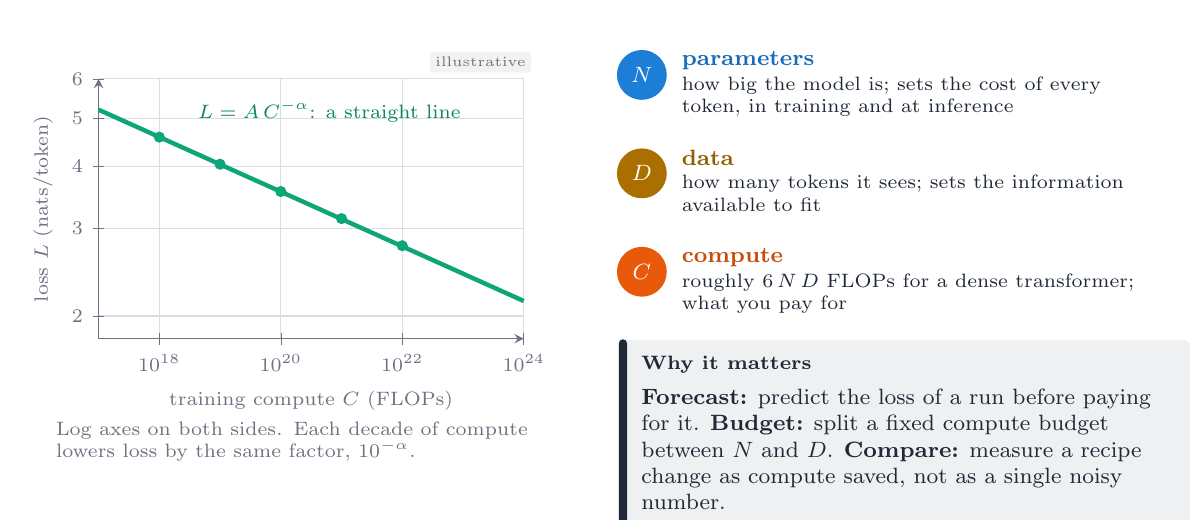
\begin{tikzpicture}
  \useasboundingbox (0,0) rectangle (14.4,5.9);
  \begin{axis}[lecture,at={(0.9cm,1.95cm)},anchor=south west,scale only axis,width=5.4cm,height=3.3cm,
      xmode=log,ymode=log,xmin=1e17,xmax=1e24,ymin=1.8,ymax=6,domain=1e17:1e24,samples=40,
      xlabel={training compute $C$ (FLOPs)},ylabel={loss $L$ (nats/token)},
      ytick={2,3,4,5,6},yticklabels={2,3,4,5,6},xtick={1e18,1e20,1e22,1e24}]
    \addplot[emb,line width=1.6pt] {5.2*(x/1e17)^(-0.055)};
    \addplot[only marks,mark=*,mark size=1.8pt,emb] coordinates {(1e18,4.58)(1e19,4.04)(1e20,3.56)(1e21,3.14)(1e22,2.77)};
    \node[font=\scriptsize,text=emb!80!black,anchor=south west] at (axis cs:3e18,4.7) {$L=A\,C^{-\alpha}$: a straight line};
  \end{axis}
  \srctag{6.4}{5.6}{illustrative}
  \node[lab,anchor=north west,text width=6.0cm] at (0.3,0.95) {Log axes on both sides. Each decade of compute lowers loss by the same factor, $10^{-\alpha}$.};
  % three resources
  \foreach \y/\sym/\name/\body/\c in {
      5.6/N/{parameters}/{how big the model is; sets the cost of every token, in training and at inference}/mlp,
      4.35/D/{data}/{how many tokens it sees; sets the information available to fit}/kct,
      3.1/C/{compute}/{roughly $6\,N\,D$ FLOPs for a dense transformer; what you pay for}/attn}{
    \node[circle,fill=\c,text=white,font=\footnotesize\bfseries,minimum size=18pt,inner sep=0] at (7.8,\y-0.3) {$\sym$};
    \node[anchor=north west,font=\footnotesize\bfseries,text=\c!85!black,inner sep=0] at (8.3,\y) {\name};
    \node[txt,anchor=north west,text width=5.9cm,font=\scriptsize] at (8.3,\y-0.32) {\body};}
  \bgpanel{7.5}{1.95}{6.7cm}{Why it matters}{%
    \hl{ink}{Forecast:} predict the loss of a run before paying for it.
    \hl{ink}{Budget:} split a fixed compute budget between $N$ and $D$.
    \hl{ink}{Compare:} measure a recipe change as compute saved, not as a
    single noisy number.}
\end{tikzpicture}
\end{frame}

% ---------------------------------------------------------------- 3
\begin{frame}{Reading a log-log plot}
\framesubtitle{A pure power law is a line whose slope is the exponent. A floor bends it, and subtracting the floor straightens it again.}
\centering
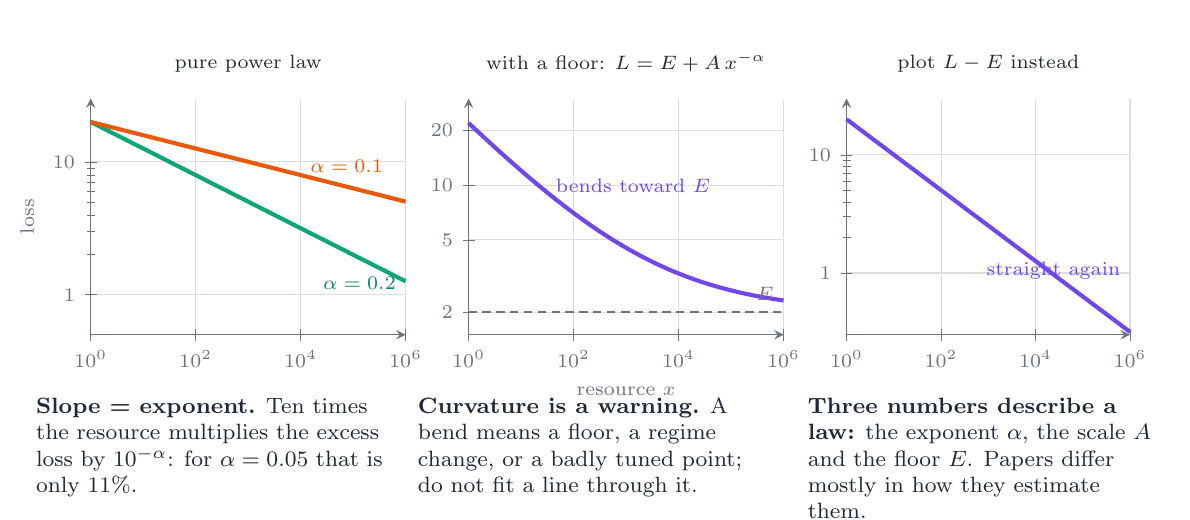
\begin{tikzpicture}
  \useasboundingbox (0,0) rectangle (14.4,5.9);
  \begin{axis}[lecture,at={(0.8cm,2.0cm)},anchor=south west,scale only axis,width=4.0cm,height=3.0cm,
      xmode=log,ymode=log,xmin=1,xmax=1e6,ymin=0.5,ymax=30,domain=1:1e6,samples=50,
      ylabel={loss},title={\scriptsize pure power law},title style={text=ink},
      xtick={1,100,10000,1000000},ytick={1,10},yticklabels={1,10}]
    \addplot[emb,line width=1.5pt] {20*x^(-0.2)};
    \addplot[attn,line width=1.5pt] {20*x^(-0.1)};
    \node[font=\scriptsize,text=emb!80!black,anchor=north east] at (axis cs:1e6,1.6) {$\alpha=0.2$};
    \node[font=\scriptsize,text=attn,anchor=south west] at (axis cs:1e4,7.0) {$\alpha=0.1$};
  \end{axis}
  \begin{axis}[lecture,at={(5.6cm,2.0cm)},anchor=south west,scale only axis,width=4.0cm,height=3.0cm,
      xmode=log,ymode=log,xmin=1,xmax=1e6,ymin=1.5,ymax=30,domain=1:1e6,samples=60,
      xlabel={resource $x$},title={\scriptsize with a floor: $L=E+A\,x^{-\alpha}$},title style={text=ink},
      xtick={1,100,10000,1000000},ytick={2,5,10,20},yticklabels={2,5,10,20}]
    \addplot[posc,line width=1.5pt] {2+20*x^(-0.3)};
    \addplot[muted,densely dashed,line width=0.7pt] {2};
    \node[font=\scriptsize,text=muted,anchor=south east] at (axis cs:1e6,2.05) {$E$};
    \node[font=\scriptsize,text=posc,anchor=south west] at (axis cs:30,8) {bends toward $E$};
  \end{axis}
  \begin{axis}[lecture,at={(10.4cm,2.0cm)},anchor=south west,scale only axis,width=3.6cm,height=3.0cm,
      xmode=log,ymode=log,xmin=1,xmax=1e6,ymin=0.3,ymax=30,domain=1:1e6,samples=50,
      title={\scriptsize plot $L-E$ instead},title style={text=ink},
      xtick={1,100,10000,1000000},ytick={1,10},yticklabels={1,10}]
    \addplot[posc,line width=1.5pt] {20*x^(-0.3)};
    \node[font=\scriptsize,text=posc,anchor=north east] at (axis cs:1e6,1.5) {straight again};
  \end{axis}
  \node[txt,anchor=north west,text width=4.4cm] at (0.1,1.2) {%
    \hl{ink}{Slope = exponent.} Ten times the resource multiplies the
    excess loss by $10^{-\alpha}$: for $\alpha=0.05$ that is only 11\%.};
  \node[txt,anchor=north west,text width=4.4cm] at (4.95,1.2) {%
    \hl{ink}{Curvature is a warning.} A bend means a floor, a regime change,
    or a badly tuned point; do not fit a line through it.};
  \node[txt,anchor=north west,text width=4.4cm] at (9.9,1.2) {%
    \hl{ink}{Three numbers describe a law:} the exponent $\alpha$, the
    scale $A$ and the floor $E$. Papers differ mostly in how they estimate
    them.};
\end{tikzpicture}
\end{frame}

% ---------------------------------------------------------------- 4
\stage{2}
\begin{frame}{History I: learning curves, 1990s}
\framesubtitle{Long before transformers, statisticians fit power laws to error versus training-set size and extrapolated them.}
\centering
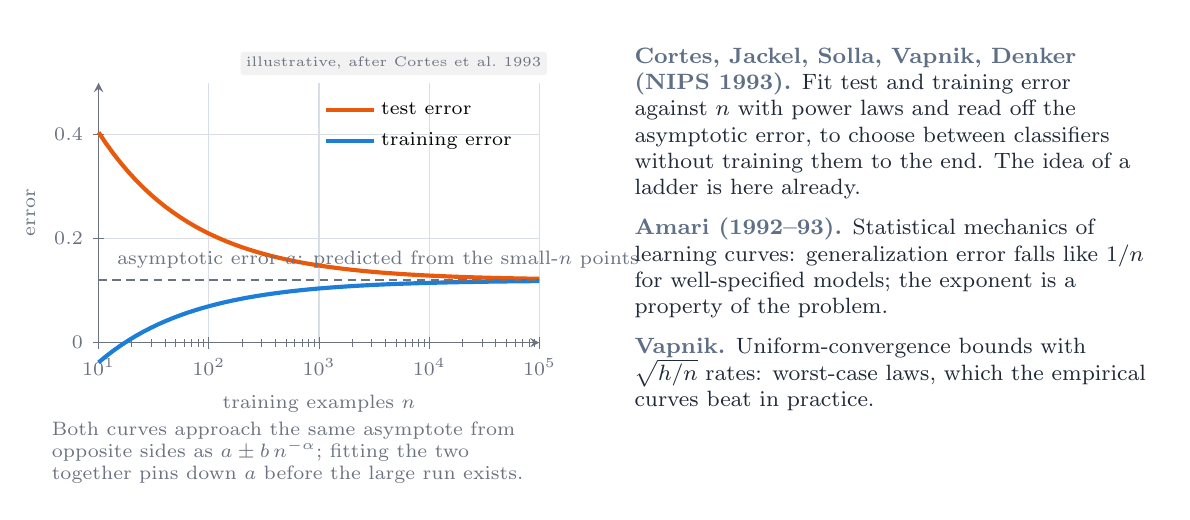
\begin{tikzpicture}
  \useasboundingbox (0,0) rectangle (14.4,5.9);
  \begin{axis}[lecture,at={(0.9cm,1.9cm)},anchor=south west,scale only axis,width=5.6cm,height=3.3cm,
      xmode=log,xmin=10,xmax=1e5,ymin=0,ymax=0.5,domain=10:1e5,samples=60,
      xlabel={training examples $n$},ylabel={error},legend pos=north east]
    \addplot[attn,line width=1.5pt] {0.12+0.9*x^(-0.5)}; \addlegendentry{test error}
    \addplot[mlp,line width=1.5pt] {0.12-0.5*x^(-0.5)}; \addlegendentry{training error}
    \addplot[muted,densely dashed,line width=0.7pt] {0.12};
    \node[font=\scriptsize,text=muted,anchor=south west] at (axis cs:12,0.125) {asymptotic error $a$: predicted from the small-$n$ points};
  \end{axis}
  \srctag{6.6}{5.6}{illustrative, after Cortes et al.\ 1993}
  \node[txt,anchor=north west,text width=6.2cm,font=\scriptsize,text=muted] at (0.3,0.9)
    {Both curves approach the same asymptote from opposite sides as $a\pm b\,n^{-\alpha}$; fitting the two together pins down $a$ before the large run exists.};
  \node[txt,anchor=north west,text width=6.5cm] at (7.7,5.65) {%
    \hl{tok}{Cortes, Jackel, Solla, Vapnik, Denker (NIPS 1993).} Fit test and
    training error against $n$ with power laws and read off the asymptotic
    error, to choose between classifiers without training them to the end.
    The idea of a ladder is here already.\\[5pt]
    \hl{tok}{Amari (1992--93).} Statistical mechanics of learning curves:
    generalization error falls like $1/n$ for well-specified models; the exponent
    is a property of the problem.\\[5pt]
    \hl{tok}{Vapnik.} Uniform-convergence bounds with $\sqrt{h/n}$ rates: worst-case
    laws, which the empirical curves beat in practice.};
\end{tikzpicture}
\end{frame}

% ---------------------------------------------------------------- 5
\begin{frame}{History II: more data beats cleverer algorithms, 2001--2017}
\framesubtitle{In NLP and then vision, accuracy kept rising log-linearly with data over three decades, for every learner tried.}
\centering
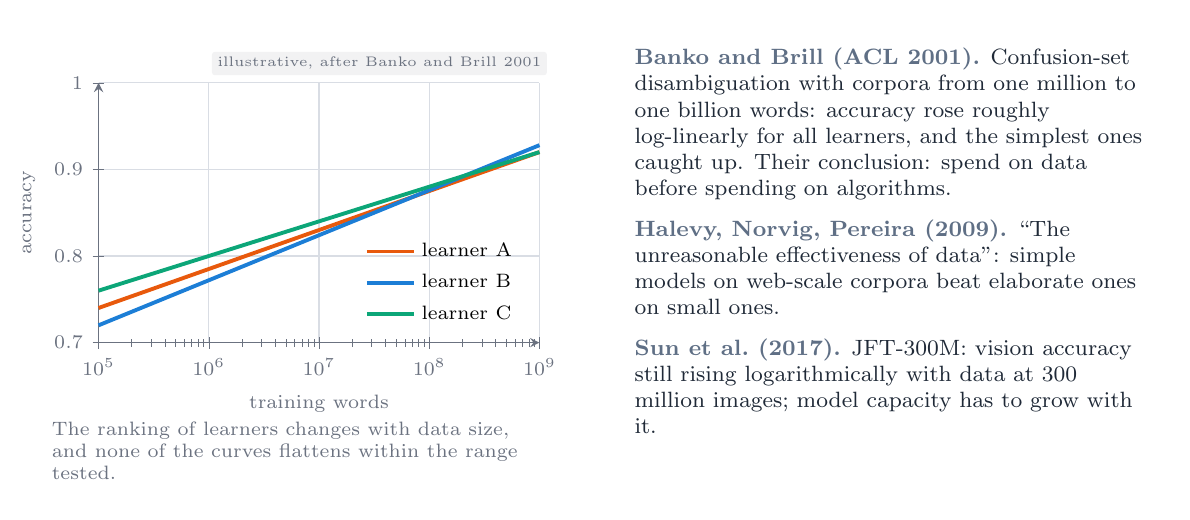
\begin{tikzpicture}
  \useasboundingbox (0,0) rectangle (14.4,5.9);
  \begin{axis}[lecture,at={(0.9cm,1.9cm)},anchor=south west,scale only axis,width=5.6cm,height=3.3cm,
      xmode=log,xmin=1e5,xmax=1e9,ymin=0.7,ymax=1.0,domain=1e5:1e9,samples=40,
      xlabel={training words},ylabel={accuracy},legend pos=south east,
      ytick={0.7,0.8,0.9,1.0}]
    \addplot[attn,line width=1.4pt] {0.74+0.045*ln(x/1e5)/ln(10)}; \addlegendentry{learner A}
    \addplot[mlp,line width=1.4pt] {0.72+0.052*ln(x/1e5)/ln(10)}; \addlegendentry{learner B}
    \addplot[emb,line width=1.4pt] {0.76+0.040*ln(x/1e5)/ln(10)}; \addlegendentry{learner C}
  \end{axis}
  \srctag{6.6}{5.6}{illustrative, after Banko and Brill 2001}
  \node[txt,anchor=north west,text width=6.2cm,font=\scriptsize,text=muted] at (0.3,0.9)
    {The ranking of learners changes with data size, and none of the curves flattens within the range tested.};
  \node[txt,anchor=north west,text width=6.5cm] at (7.7,5.65) {%
    \hl{tok}{Banko and Brill (ACL 2001).} Confusion-set disambiguation with
    corpora from one million to one billion words: accuracy rose roughly
    log-linearly for all learners, and the simplest ones caught up. Their
    conclusion: spend on data before spending on algorithms.\\[5pt]
    \hl{tok}{Halevy, Norvig, Pereira (2009).} ``The unreasonable effectiveness
    of data'': simple models on web-scale corpora beat elaborate ones on small
    ones.\\[5pt]
    \hl{tok}{Sun et al.\ (2017).} JFT-300M: vision accuracy still rising
    logarithmically with data at 300 million images; model capacity has to grow
    with it.};
\end{tikzpicture}
\end{frame}

% ---------------------------------------------------------------- 6
\begin{frame}{History III: deep learning scaling is predictable, 2017--2019}
\framesubtitle{Hestness et al.\ measured learning curves across domains: the same three-region shape, with task-specific exponents.}
\centering
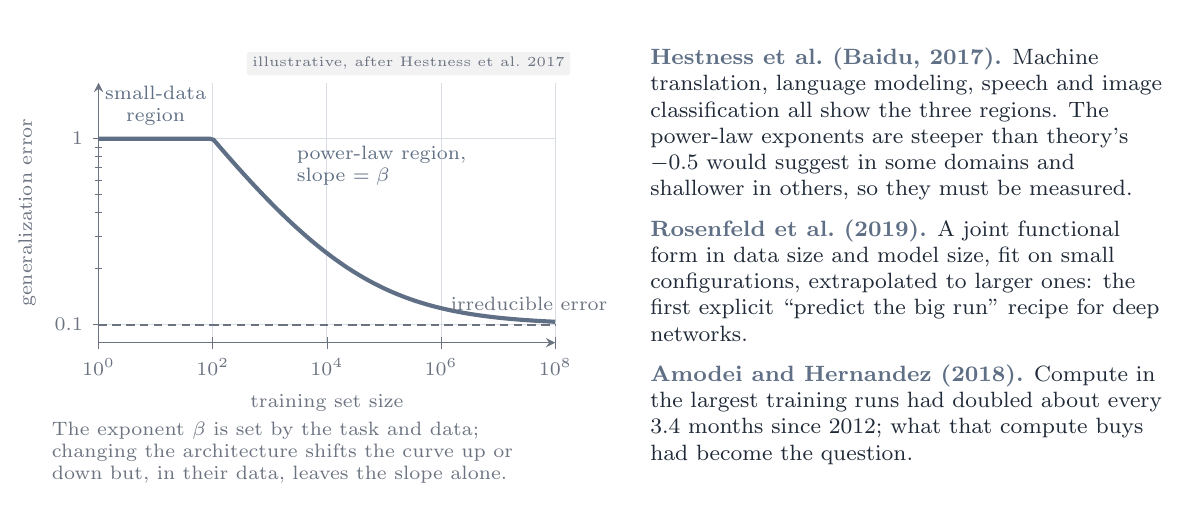
\begin{tikzpicture}
  \useasboundingbox (0,0) rectangle (14.4,5.9);
  \begin{axis}[lecture,at={(0.9cm,1.9cm)},anchor=south west,scale only axis,width=5.8cm,height=3.3cm,
      xmode=log,ymode=log,xmin=1,xmax=1e8,ymin=0.08,ymax=2,domain=1:1e8,samples=120,
      xlabel={training set size},ylabel={generalization error},
      ytick={0.1,1},yticklabels={0.1,1},xtick={1,100,10000,1000000,100000000}]
    \addplot[tok,line width=1.5pt] {0.1+0.9*min(1,(x/100)^(-0.4))};
    \addplot[muted,densely dashed,line width=0.7pt] {0.1};
    \node[font=\scriptsize,text=tok,anchor=south,align=center] at (axis cs:10,1.05) {small-data\\region};
    \node[font=\scriptsize,text=tok,anchor=south west,align=left] at (axis cs:2000,0.5) {power-law region,\\slope $=\beta$};
    \node[font=\scriptsize,text=muted,anchor=south west] at (axis cs:1e6,0.105) {irreducible error};
  \end{axis}
  \srctag{6.9}{5.6}{illustrative, after Hestness et al.\ 2017}
  \node[txt,anchor=north west,text width=6.3cm,font=\scriptsize,text=muted] at (0.3,0.9)
    {The exponent $\beta$ is set by the task and data; changing the architecture shifts the curve up or down but, in their data, leaves the slope alone.};
  \node[txt,anchor=north west,text width=6.5cm] at (7.9,5.65) {%
    \hl{tok}{Hestness et al.\ (Baidu, 2017).} Machine translation, language
    modeling, speech and image classification all show the three regions. The
    power-law exponents are steeper than theory's $-0.5$ would suggest in
    some domains and shallower in others, so they must be measured.\\[5pt]
    \hl{tok}{Rosenfeld et al.\ (2019).} A joint functional form in data size
    and model size, fit on small configurations, extrapolated to larger ones:
    the first explicit ``predict the big run'' recipe for deep networks.\\[5pt]
    \hl{tok}{Amodei and Hernandez (2018).} Compute in the largest training runs
    had doubled about every 3.4 months since 2012; what that compute buys had
    become the question.};
\end{tikzpicture}
\end{frame}

% ---------------------------------------------------------------- 7
\stage{3}
\begin{frame}{Kaplan et al.\ 2020: three laws for language models}
\framesubtitle{Loss is a power law in each of parameters, data and compute when the other two are not the bottleneck.}
\centering
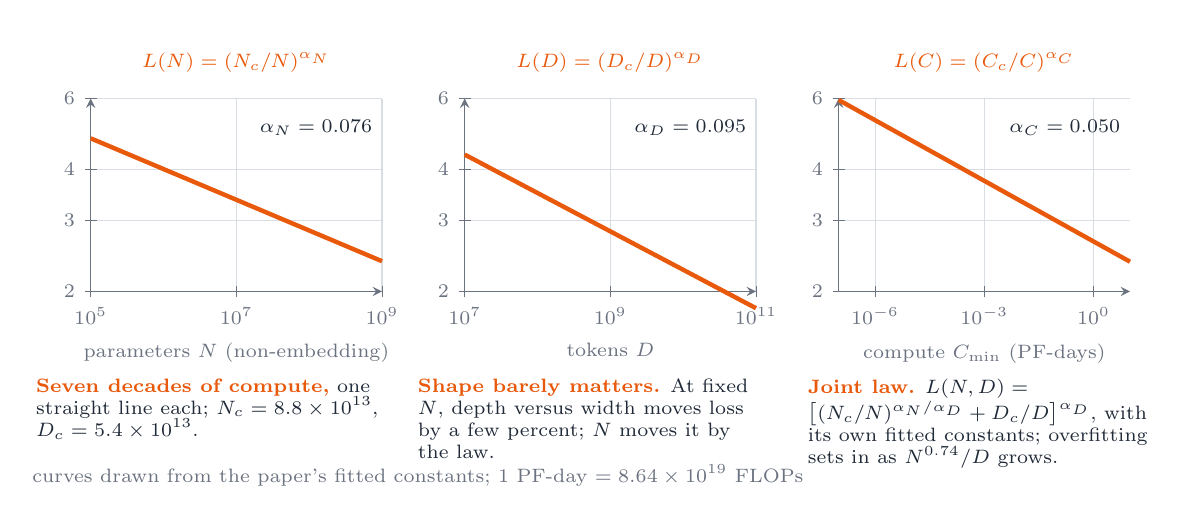
\begin{tikzpicture}
  \useasboundingbox (0,0) rectangle (14.4,5.9);
  \begin{axis}[lecture,at={(0.8cm,2.55cm)},anchor=south west,scale only axis,width=3.7cm,height=2.45cm,
      xmode=log,ymode=log,xmin=1e5,xmax=1e9,ymin=2,ymax=6,domain=1e5:1e9,samples=40,
      xlabel={parameters $N$ (non-embedding)},ytick={2,3,4,6},yticklabels={2,3,4,6},xtick={1e5,1e7,1e9},
      title={\scriptsize $L(N)=(N_c/N)^{\alpha_N}$},title style={text=attn}]
    \addplot[attn,line width=1.6pt] {(8.8e13/x)^0.076};
    \node[font=\scriptsize,text=ink,anchor=north east] at (axis cs:1e9,5.6) {$\alpha_N=0.076$};
  \end{axis}
  \begin{axis}[lecture,at={(5.55cm,2.55cm)},anchor=south west,scale only axis,width=3.7cm,height=2.45cm,
      xmode=log,ymode=log,xmin=1e7,xmax=1e11,ymin=2,ymax=6,domain=1e7:1e11,samples=40,
      xlabel={tokens $D$},ytick={2,3,4,6},yticklabels={2,3,4,6},xtick={1e7,1e9,1e11},
      title={\scriptsize $L(D)=(D_c/D)^{\alpha_D}$},title style={text=attn}]
    \addplot[attn,line width=1.6pt] {(5.4e13/x)^0.095};
    \node[font=\scriptsize,text=ink,anchor=north east] at (axis cs:1e11,5.6) {$\alpha_D=0.095$};
  \end{axis}
  \begin{axis}[lecture,at={(10.3cm,2.55cm)},anchor=south west,scale only axis,width=3.7cm,height=2.45cm,
      xmode=log,ymode=log,xmin=1e-7,xmax=10,ymin=2,ymax=6,domain=1e-7:10,samples=40,
      xlabel={compute $C_{\min}$ (PF-days)},ytick={2,3,4,6},yticklabels={2,3,4,6},xtick={1e-6,1e-3,1},
      title={\scriptsize $L(C)=(C_c/C)^{\alpha_C}$},title style={text=attn}]
    \addplot[attn,line width=1.6pt] {(3.1e8/x)^0.050};
    \node[font=\scriptsize,text=ink,anchor=north east] at (axis cs:10,5.6) {$\alpha_C=0.050$};
  \end{axis}
  \node[lab,anchor=south west] at (0.0,0.02) {curves drawn from the paper's fitted constants; 1 PF-day $=8.64\times10^{19}$ FLOPs};
  \node[txt,anchor=north west,text width=4.4cm,font=\scriptsize] at (0.1,1.45) {%
    \hl{attn}{Seven decades of compute,} one straight line each;
    $N_c=8.8\times10^{13}$, $D_c=5.4\times10^{13}$.};
  \node[txt,anchor=north west,text width=4.4cm,font=\scriptsize] at (4.95,1.45) {%
    \hl{attn}{Shape barely matters.} At fixed $N$, depth versus width moves
    loss by a few percent; $N$ moves it by the law.};
  \node[txt,anchor=north west,text width=4.4cm,font=\scriptsize] at (9.9,1.45) {%
    \hl{attn}{Joint law.} $L(N,D)=\big[(N_c/N)^{\alpha_N/\alpha_D}+D_c/D\big]^{\alpha_D}$,
    with its own fitted constants; overfitting sets in as $N^{0.74}/D$ grows.};
\end{tikzpicture}
\end{frame}

% ---------------------------------------------------------------- 8
\begin{frame}{Kaplan's recipe: grow the model faster than the data}
\framesubtitle{Allocating a growing budget by the 2020 fits sends most of each new decade of compute to parameters, not tokens.}
\centering
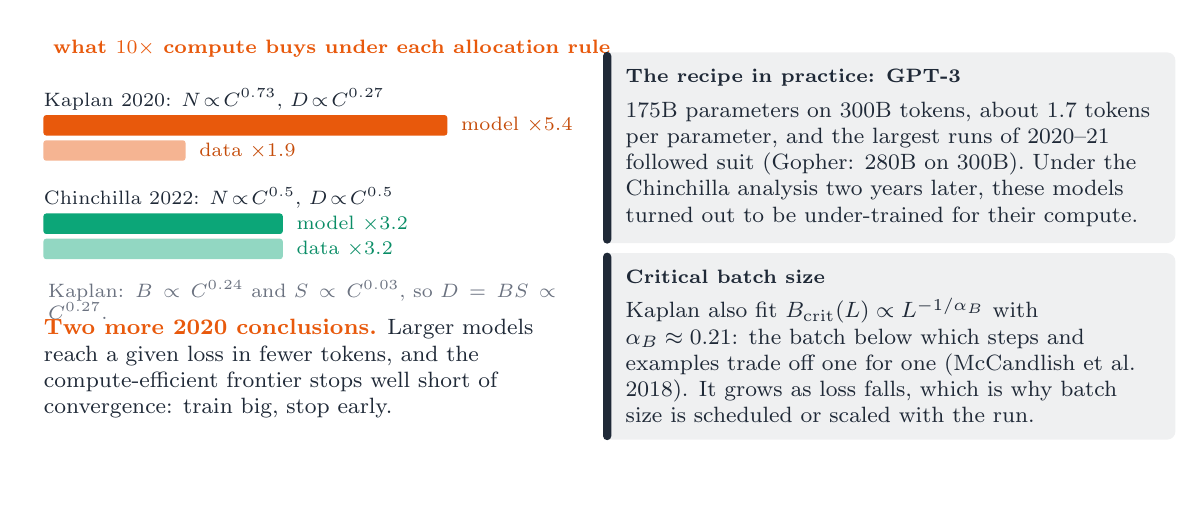
\begin{tikzpicture}
  \useasboundingbox (0,0) rectangle (14.4,5.9);
  % allocation for 10x compute
  \node[font=\scriptsize\bfseries,text=attn,anchor=south west] at (0.2,5.4) {what $10\times$ compute buys under each allocation rule};
  \foreach \y/\lab/\n/\d/\c in {4.55/{Kaplan 2020: $N\!\propto\!C^{0.73}$, $D\!\propto\!C^{0.27}$}/5.4/1.9/attn,
                               3.3/{Chinchilla 2022: $N\!\propto\!C^{0.5}$, $D\!\propto\!C^{0.5}$}/3.2/3.2/emb}{
    \node[anchor=south west,font=\scriptsize,text=ink,inner sep=0] at (0.2,\y+0.3) {\lab};
    \fill[\c,rounded corners=1pt] (0.2,\y-0.02) rectangle ++({\n*0.95},0.26);
    \node[anchor=west,font=\scriptsize,text=\c!85!black] at ({0.25+\n*0.95},\y+0.11) {model $\times\n$};
    \fill[\c!45,rounded corners=1pt] (0.2,\y-0.34) rectangle ++({\d*0.95},0.26);
    \node[anchor=west,font=\scriptsize,text=\c!85!black] at ({0.25+\d*0.95},\y-0.21) {data $\times\d$};}
  \node[lab,anchor=north west,text width=6.8cm] at (0.2,2.75) {Kaplan: $B\propto C^{0.24}$ and $S\propto C^{0.03}$, so $D=BS\propto C^{0.27}$.};
  \node[txt,anchor=north west,text width=6.4cm] at (0.2,2.2) {%
    \hl{attn}{Two more 2020 conclusions.} Larger models reach a given loss in
    fewer tokens, and the compute-efficient frontier stops well short of
    convergence: train big, stop early.};
  \bgpanel{7.3}{5.6}{6.7cm}{The recipe in practice: GPT-3}{%
    175B parameters on 300B tokens, about 1.7 tokens per parameter, and the
    largest runs of 2020--21 followed suit (Gopher: 280B on 300B). Under the
    Chinchilla analysis two years later, these models turned out to be
    under-trained for their compute.}
  \bgpanel{7.3}{3.05}{6.7cm}{Critical batch size}{%
    Kaplan also fit $B_{\text{crit}}(L)\propto L^{-1/\alpha_B}$ with $\alpha_B\approx0.21$:
    the batch below which steps and examples trade off one for one (McCandlish et
    al.\ 2018). It grows as loss falls, which is why batch size is scheduled or
    scaled with the run.}
\end{tikzpicture}
\end{frame}

% ---------------------------------------------------------------- 9
\stage{4}
\begin{frame}{Chinchilla, 2022: three ways to find the compute-optimal split}
\framesubtitle{Over 400 models from 70M to 16B parameters, one question: at a fixed compute budget, how big should the model be?}
\centering
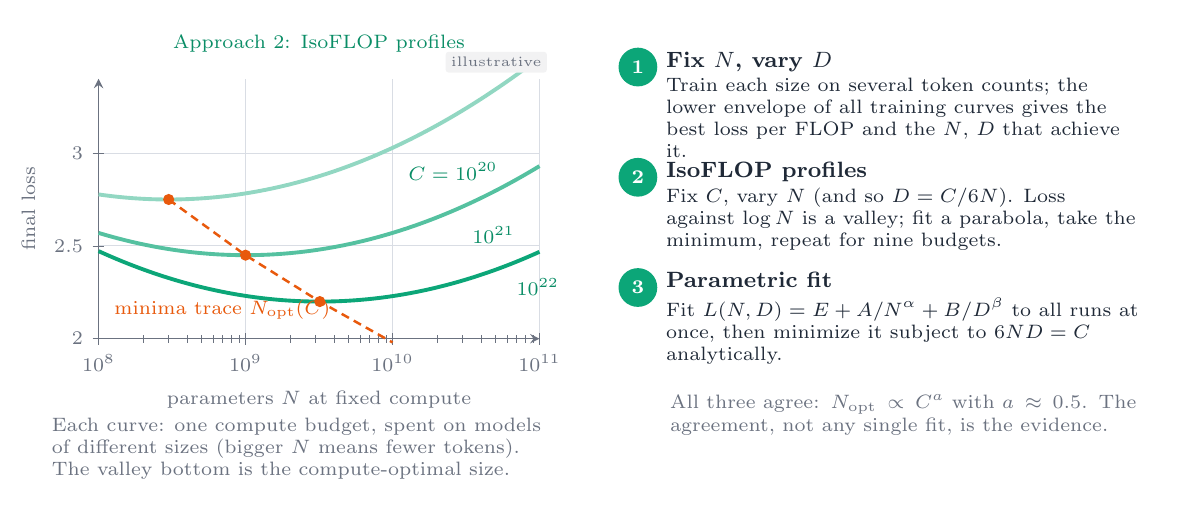
\begin{tikzpicture}
  \useasboundingbox (0,0) rectangle (14.4,5.9);
  \begin{axis}[lecture,at={(0.9cm,1.95cm)},anchor=south west,scale only axis,width=5.6cm,height=3.3cm,
      xmode=log,xmin=1e8,xmax=1e11,ymin=2.0,ymax=3.4,domain=1e8:1e11,samples=80,
      xlabel={parameters $N$ at fixed compute},ylabel={final loss},xtick={1e8,1e9,1e10,1e11},
      title={\scriptsize Approach 2: IsoFLOP profiles},title style={text=emb!85!black}]
    \addplot[emb!45,line width=1.4pt] {2.75+0.12*(ln(x/3e8)/ln(10))^2};
    \addplot[emb!70,line width=1.4pt] {2.45+0.12*(ln(x/1e9)/ln(10))^2};
    \addplot[emb,line width=1.4pt] {2.2+0.12*(ln(x/3.2e9)/ln(10))^2};
    \addplot[attn,densely dashed,line width=0.9pt] coordinates {(3e8,2.75)(1e9,2.45)(3.2e9,2.2)(1e10,1.98)};
    \addplot[only marks,mark=*,mark size=1.8pt,attn] coordinates {(3e8,2.75)(1e9,2.45)(3.2e9,2.2)};
    \node[font=\scriptsize,text=emb!85!black,anchor=west] at (axis cs:1.1e10,2.9) {$C=10^{20}$};
    \node[font=\scriptsize,text=emb!85!black,anchor=west] at (axis cs:3e10,2.56) {$10^{21}$};
    \node[font=\scriptsize,text=emb!85!black,anchor=west] at (axis cs:6e10,2.28) {$10^{22}$};
    \node[font=\scriptsize,text=attn,anchor=south west] at (axis cs:1.1e8,2.05) {minima trace $N_{\text{opt}}(C)$};
  \end{axis}
  \srctag{6.6}{5.6}{illustrative}
  \node[txt,anchor=north west,text width=6.3cm,font=\scriptsize,text=muted] at (0.3,0.95)
    {Each curve: one compute budget, spent on models of different sizes (bigger $N$ means fewer tokens). The valley bottom is the compute-optimal size.};
  \foreach \y/\num/\ttl/\body in {
      5.6/1/{Fix $N$, vary $D$}/{Train each size on several token counts; the lower envelope of all training curves gives the best loss per FLOP and the $N$, $D$ that achieve it.},
      4.2/2/{IsoFLOP profiles}/{Fix $C$, vary $N$ (and so $D=C/6N$). Loss against $\log N$ is a valley; fit a parabola, take the minimum, repeat for nine budgets.},
      2.8/3/{Parametric fit}/{Fit $L(N,D)=E+A/N^{\alpha}+B/D^{\beta}$ to all runs at once, then minimize it subject to $6ND=C$ analytically.}}{
    \node[circle,fill=emb,text=white,font=\scriptsize\bfseries,inner sep=0pt,minimum size=14pt] at (7.75,\y-0.2) {\num};
    \node[anchor=north west,font=\footnotesize\bfseries,text=ink,inner sep=0] at (8.1,\y) {\ttl};
    \node[txt,anchor=north west,text width=6.0cm,font=\scriptsize] at (8.1,\y-0.33) {\body};}
  \node[lab,anchor=north west,text width=6.3cm] at (8.1,1.3) {All three agree: $N_{\text{opt}}\propto C^{a}$ with $a\approx0.5$. The agreement, not any single fit, is the evidence.};
\end{tikzpicture}
\end{frame}

% ---------------------------------------------------------------- 10
\begin{frame}{Chinchilla's result: scale parameters and tokens together}
\framesubtitle{About twenty tokens per parameter at the compute-optimal point, and a 70B model that beat a 280B one at equal cost.}
\centering
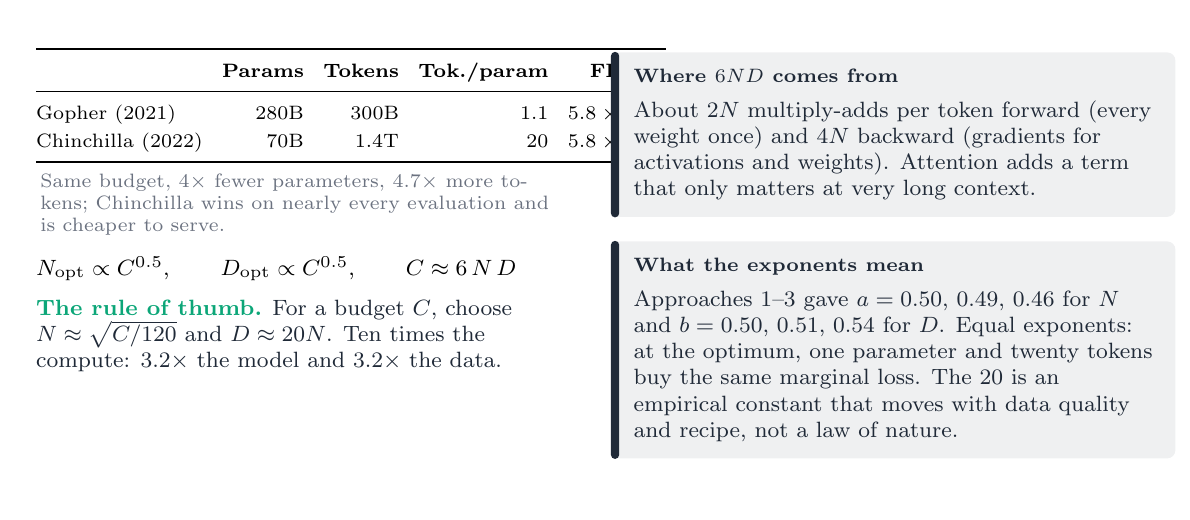
\begin{tikzpicture}
  \useasboundingbox (0,0) rectangle (14.4,5.9);
  \node[anchor=north west,inner sep=0,font=\fontsize{6.8}{8.5}\selectfont] at (0.1,5.65) {%
    \renewcommand{\arraystretch}{1.2}\setlength{\tabcolsep}{3.5pt}%
    \begin{tabular}{@{}lrrrr@{}}
      \toprule
      & \textbf{Params} & \textbf{Tokens} & \textbf{Tok./param} & \textbf{FLOPs}\\
      \midrule
      Gopher (2021)     & 280B & 300B & 1.1 & $5.8\times10^{23}$\\
      Chinchilla (2022) & 70B  & 1.4T & 20  & $5.8\times10^{23}$\\
      \bottomrule
    \end{tabular}};
  \node[lab,anchor=north west,text width=6.9cm] at (0.1,4.1) {Same budget, 4$\times$ fewer parameters, 4.7$\times$ more tokens; Chinchilla wins on nearly every evaluation and is cheaper to serve.};
  \node[anchor=north west,inner sep=0,font=\footnotesize] at (0.1,3.0)
    {$N_{\text{opt}}\propto C^{0.5},\qquad D_{\text{opt}}\propto C^{0.5},\qquad C\approx 6\,N\,D$};
  \node[txt,anchor=north west,text width=6.9cm] at (0.1,2.45) {%
    \hl{emb}{The rule of thumb.} For a budget $C$, choose $N\approx\sqrt{C/120}$
    and $D\approx20N$. Ten times the compute: $3.2\times$ the model and
    $3.2\times$ the data.};
  \bgpanel{7.4}{5.6}{6.6cm}{Where $6ND$ comes from}{%
    About $2N$ multiply-adds per token forward (every weight once) and $4N$
    backward (gradients for activations and weights). Attention adds a term
    that only matters at very long context.}
  \bgpanel{7.4}{3.2}{6.6cm}{What the exponents mean}{%
    Approaches 1--3 gave $a=0.50,\,0.49,\,0.46$ for $N$ and $b=0.50,\,0.51,\,0.54$
    for $D$. Equal exponents: at the optimum, one parameter and twenty tokens buy
    the same marginal loss. The 20 is an empirical constant that moves with data
    quality and recipe, not a law of nature.}
\end{tikzpicture}
\end{frame}

% ---------------------------------------------------------------- 11
\begin{frame}{Why Kaplan and Chinchilla disagreed}
\framesubtitle{Same question, exponents of 0.73 versus 0.5. The gap is methodology, and later papers pinned down each piece.}
\centering
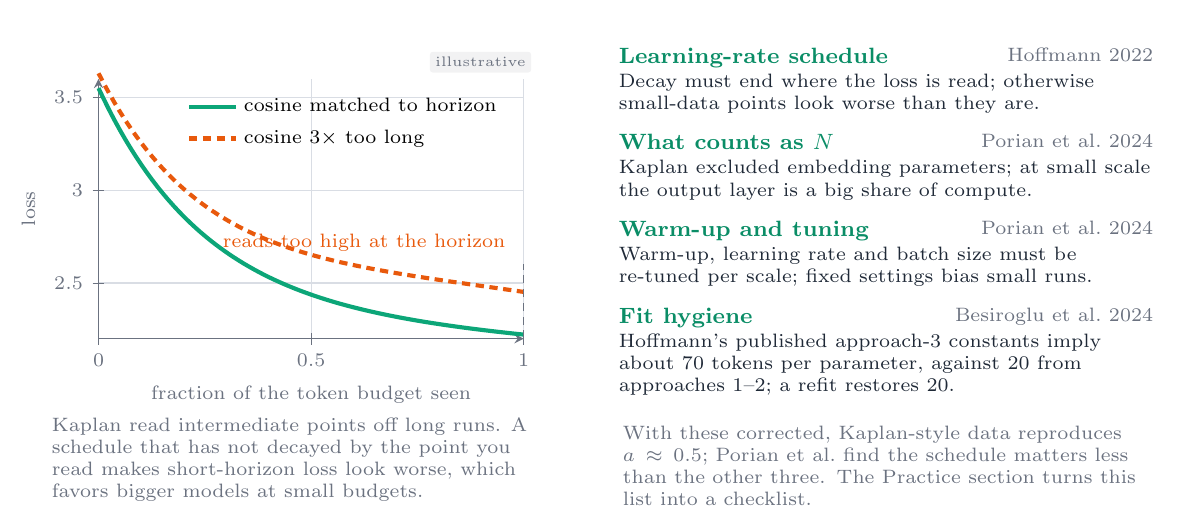
\begin{tikzpicture}
  \useasboundingbox (0,0) rectangle (14.4,5.9);
  \begin{axis}[lecture,at={(0.9cm,1.95cm)},anchor=south west,scale only axis,width=5.4cm,height=3.3cm,
      xmin=0,xmax=1,ymin=2.2,ymax=3.6,domain=0:1,samples=80,
      xlabel={fraction of the token budget seen},ylabel={loss},legend pos=north east,xtick={0,0.5,1}]
    \addplot[emb,line width=1.5pt] {2.35+1.2*exp(-4*x)-0.15*x}; \addlegendentry{cosine matched to horizon}
    \addplot[attn,line width=1.5pt,densely dashed] {2.35+1.2*exp(-4*x)+0.12*x*(1-x)*2+0.08}; \addlegendentry{cosine 3$\times$ too long}
    \draw[muted,densely dashed] (axis cs:1,2.2) -- (axis cs:1,2.6);
    \node[font=\scriptsize,text=attn,anchor=south east] at (axis cs:0.98,2.62) {reads too high at the horizon};
  \end{axis}
  \srctag{6.4}{5.6}{illustrative}
  \node[txt,anchor=north west,text width=6.1cm,font=\scriptsize,text=muted] at (0.3,0.95)
    {Kaplan read intermediate points off long runs. A schedule that has not decayed by the point you read makes short-horizon loss look worse, which favors bigger models at small budgets.};
  \foreach \y/\ttl/\body/\who in {
      5.65/{Learning-rate schedule}/{Decay must end where the loss is read; otherwise small-data points look worse than they are.}/{Hoffmann 2022},
      4.55/{What counts as $N$}/{Kaplan excluded embedding parameters; at small scale the output layer is a big share of compute.}/{Porian et al.\ 2024},
      3.45/{Warm-up and tuning}/{Warm-up, learning rate and batch size must be re-tuned per scale; fixed settings bias small runs.}/{Porian et al.\ 2024},
      2.35/{Fit hygiene}/{Hoffmann's published approach-3 constants imply about 70 tokens per parameter, against 20 from approaches 1--2; a refit restores 20.}/{Besiroglu et al.\ 2024}}{
    \node[anchor=north west,font=\footnotesize\bfseries,text=emb!85!black,inner sep=0] at (7.5,\y) {\ttl};
    \node[anchor=north east,font=\scriptsize,text=muted,inner sep=0] at (14.3,\y) {\who};
    \node[txt,anchor=north west,text width=6.8cm,font=\scriptsize] at (7.5,\y-0.33) {\body};}
  \node[lab,anchor=north west,text width=6.8cm] at (7.5,0.9) {With these corrected, Kaplan-style data reproduces $a\approx0.5$; Porian et al.\ find the schedule matters less than the other three. The Practice section turns this list into a checklist.};
\end{tikzpicture}
\end{frame}

% ---------------------------------------------------------------- 12
\begin{frame}{The parametric form, term by term}
\framesubtitle{$L(N,D)=E+A/N^{\alpha}+B/D^{\beta}$ is the workhorse. Each term has a meaning, and the fit has a standard procedure.}
\centering
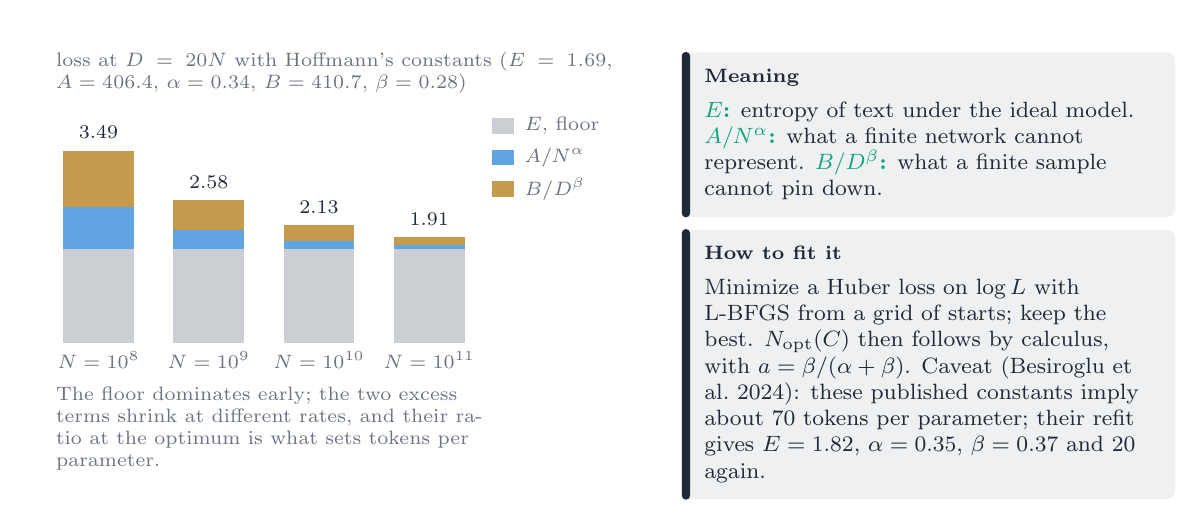
\begin{tikzpicture}
  \useasboundingbox (0,0) rectangle (14.4,5.9);
  % stacked decomposition
  \foreach \x/\N/\ta/\tb/\tot in {0.9/8/0.774/1.021/3.49,2.3/9/0.354/0.536/2.58,3.7/10/0.162/0.281/2.13,5.1/11/0.074/0.148/1.91}{
    \fill[muted!35] (\x-0.45,1.9) rectangle ++(0.9,{1.69*0.7});
    \fill[mlp!70] (\x-0.45,{1.9+1.69*0.7}) rectangle ++(0.9,{\ta*0.7});
    \fill[kct!70] (\x-0.45,{1.9+(1.69+\ta)*0.7}) rectangle ++(0.9,{\tb*0.7});
    \node[lab,anchor=north] at (\x,1.85) {$N=10^{\N}$};
    \node[font=\scriptsize,text=ink,anchor=south] at (\x,{1.9+\tot*0.7+0.03}) {\tot};}
  \node[lab,anchor=north west,text width=7.6cm] at (0.3,5.65) {loss at $D=20N$ with Hoffmann's constants ($E=1.69$, $A=406.4$, $\alpha=0.34$, $B=410.7$, $\beta=0.28$)};
  \fill[muted!35] (5.9,4.55) rectangle ++(0.28,0.2); \node[lab,anchor=west] at (6.25,4.65) {$E$, floor};
  \fill[mlp!70] (5.9,4.15) rectangle ++(0.28,0.2); \node[lab,anchor=west] at (6.25,4.25) {$A/N^{\alpha}$};
  \fill[kct!70] (5.9,3.75) rectangle ++(0.28,0.2); \node[lab,anchor=west] at (6.25,3.85) {$B/D^{\beta}$};
  \node[lab,anchor=north west,text width=5.6cm] at (0.3,1.4) {The floor dominates early; the two excess terms shrink at different rates, and their ratio at the optimum is what sets tokens per parameter.};
  \bgpanel{8.3}{5.6}{5.7cm}{Meaning}{%
    \hl{emb}{$E$:} entropy of text under the ideal model.
    \hl{emb}{$A/N^{\alpha}$:} what a finite network cannot represent.
    \hl{emb}{$B/D^{\beta}$:} what a finite sample cannot pin down.}
  \bgpanel{8.3}{3.35}{5.7cm}{How to fit it}{%
    Minimize a Huber loss on $\log L$ with L-BFGS from a grid of starts; keep
    the best. $N_{\text{opt}}(C)$ then follows by calculus, with
    $a=\beta/(\alpha+\beta)$. Caveat (Besiroglu et al.\ 2024): these published
    constants imply about 70 tokens per parameter; their refit gives
    $E=1.82$, $\alpha=0.35$, $\beta=0.37$ and 20 again.}
\end{tikzpicture}
\end{frame}

% ---------------------------------------------------------------- 12b
\begin{frame}{Why power laws at all?}
\framesubtitle{Three pictures that produce them, each saying what the exponent depends on. None is settled; all are useful.}
\centering
\begin{tikzpicture}
  \useasboundingbox (0,0) rectangle (14.4,5.9);
  \foreach \x/\c/\ttl/\body/\who in {
      0.1/emb/{Resolution on a manifold}/{Data lies near a $d$-dimensional manifold. $N$ parameters resolve it to spacing $\propto N^{-1/d}$; a smooth target then gives $L-E\propto N^{-4/d}$. Small exponent, high-dimensional data.}/{Sharma, Kaplan 2020; Bahri et al.\ 2021},
      4.85/attn/{Zipf-distributed features}/{Feature frequencies follow a power law. Each feature is learned once enough examples are seen, so the loss left after $D$ tokens is a power law in $D$ whose exponent is set by the Zipf slope.}/{Hutter 2021},
      9.6/posc/{Quanta of skill}/{Loss is a sum over many discrete ``skills'', each learned at its own scale and used with Zipfian frequency. Averaged, they give a smooth power law even though each one switches on abruptly.}/{Michaud et al.\ 2023}}{
    \node[anchor=north west,inner sep=0] at (\x,5.6) {%
      \begin{tikzpicture}
        \node[anchor=north west,minimum width=4.6cm,minimum height=4.1cm,rounded corners=4pt,fill=\c!8] (b) {};
        \fill[\c,rounded corners=2pt] (b.north west) rectangle ([yshift=-0.14cm]b.north east);
        \node[anchor=north west,text width=4.1cm,font=\small\bfseries,text=\c!85!black,inner sep=0] at ([xshift=8pt,yshift=-12pt]b.north west) {\ttl};
        \node[anchor=north west,text width=4.1cm,font=\scriptsize,text=ink,inner sep=0,align=flush left] at ([xshift=8pt,yshift=-30pt]b.north west) {\body};
        \node[anchor=south west,text width=4.1cm,font=\scriptsize,text=\c!85!black,inner sep=0] at ([xshift=8pt,yshift=7pt]b.south west) {\who};
      \end{tikzpicture}};}
  \node[txt,anchor=north west,text width=14.1cm] at (0.1,1.3) {%
    \hl{ink}{What they agree on.} The exponent belongs to the data
    distribution more than to the architecture: Hestness saw architectures
    shift curves without changing slopes, and a new data mix needs its own
    ladder. Bahri et al.\ also separate a variance-limited regime (exponent 1,
    when one resource dwarfs the other) from the resolution-limited one above.};
\end{tikzpicture}
\end{frame}

% ---------------------------------------------------------------- 14
\stage{5}
\begin{frame}{Refinement I: the cost of serving changes the optimum}
\framesubtitle{Chinchilla minimizes training compute. If the model will answer billions of queries, serving cost belongs in the objective.}
\centering
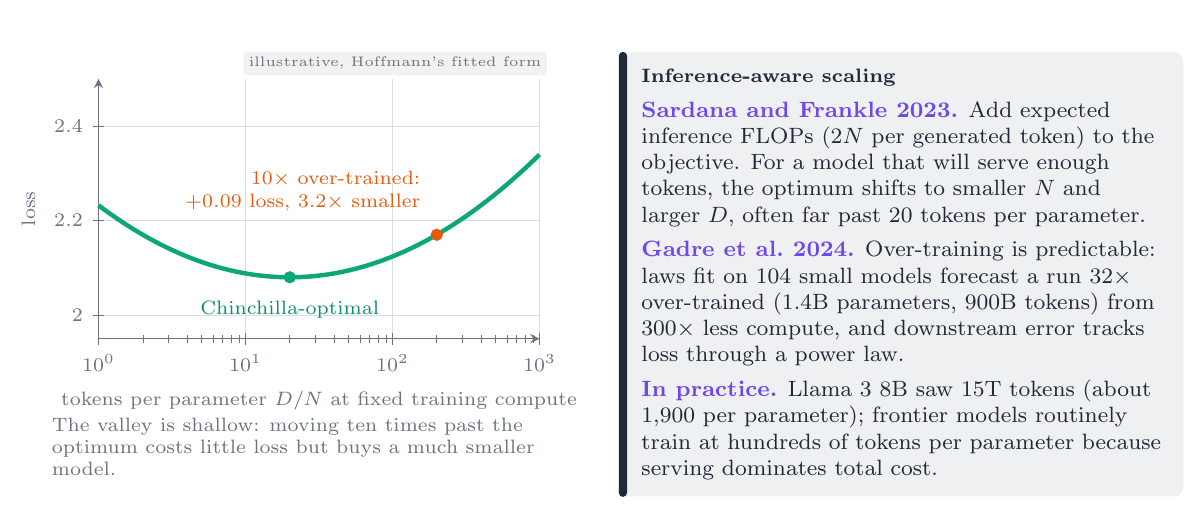
\begin{tikzpicture}
  \useasboundingbox (0,0) rectangle (14.4,5.9);
  \begin{axis}[lecture,at={(0.9cm,1.95cm)},anchor=south west,scale only axis,width=5.6cm,height=3.3cm,
      xmode=log,xmin=1,xmax=1000,ymin=1.95,ymax=2.5,domain=1:1000,samples=80,
      xlabel={tokens per parameter $D/N$ at fixed training compute},ylabel={loss},xtick={1,10,100,1000}]
    \addplot[emb,line width=1.6pt] {2.08+0.09*(ln(x/20)/ln(10))^2};
    \addplot[only marks,mark=*,mark size=2pt,emb] coordinates {(20,2.08)};
    \addplot[only marks,mark=*,mark size=2pt,attn] coordinates {(200,2.17)};
    \node[font=\scriptsize,text=emb!85!black,anchor=north] at (axis cs:20,2.05) {Chinchilla-optimal};
    \node[font=\scriptsize,text=attn,anchor=south east,align=right] at (axis cs:180,2.2) {$10\times$ over-trained:\\$+0.09$ loss, $3.2\times$ smaller};
  \end{axis}
  \srctag{6.6}{5.6}{illustrative, Hoffmann's fitted form}
  \node[txt,anchor=north west,text width=6.3cm,font=\scriptsize,text=muted] at (0.3,0.95)
    {The valley is shallow: moving ten times past the optimum costs little loss but buys a much smaller model.};
  \bgpanel{7.5}{5.6}{6.6cm}{Inference-aware scaling}{%
    \hl{posc}{Sardana and Frankle 2023.} Add expected inference FLOPs
    ($2N$ per generated token) to the objective. For a model that will serve
    enough tokens, the optimum shifts to smaller $N$ and larger $D$, often far
    past 20 tokens per parameter.\\[3pt]
    \hl{posc}{Gadre et al.\ 2024.} Over-training is predictable: laws fit on
    104 small models forecast a run $32\times$ over-trained (1.4B parameters,
    900B tokens) from $300\times$ less compute, and downstream error tracks
    loss through a power law.\\[3pt]
    \hl{posc}{In practice.} Llama 3 8B saw 15T tokens (about 1{,}900 per
    parameter); frontier models routinely train at hundreds of tokens per
    parameter because serving dominates total cost.}
\end{tikzpicture}
\end{frame}

% ---------------------------------------------------------------- 15
\begin{frame}{Refinement II: when data runs out, repeat it}
\framesubtitle{Unique text is finite. Muennighoff et al.\ measured what a repeated token is worth and fit a law with a decay constant.}
\centering
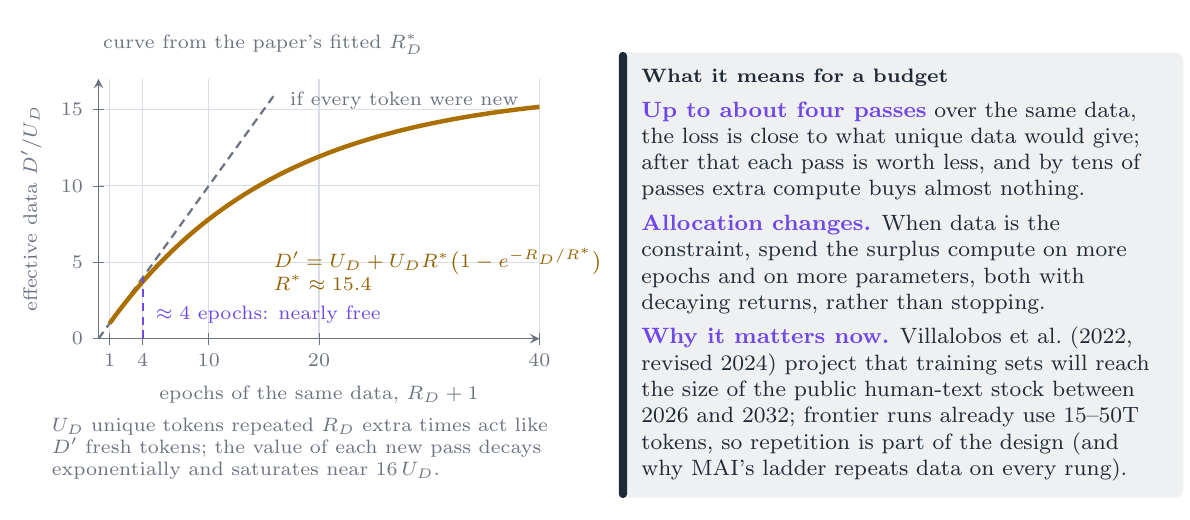
\begin{tikzpicture}
  \useasboundingbox (0,0) rectangle (14.4,5.9);
  \begin{axis}[lecture,at={(0.9cm,1.95cm)},anchor=south west,scale only axis,width=5.6cm,height=3.3cm,
      xmin=0,xmax=40,ymin=0,ymax=17,domain=1:40,samples=80,
      xlabel={epochs of the same data, $R_D+1$},ylabel={effective data $D'/U_D$},xtick={1,4,10,20,40},ytick={0,5,10,15}]
    \addplot[muted,densely dashed,line width=0.8pt,domain=0:16] {x};
    \addplot[kct,line width=1.6pt] {1+15.39*(1-exp(-(x-1)/15.39))};
    \draw[posc,densely dashed,line width=0.7pt] (axis cs:4,0) -- (axis cs:4,4);
    \node[font=\scriptsize,text=posc,anchor=south west] at (axis cs:4.3,0.4) {$\approx4$ epochs: nearly free};
    \node[font=\scriptsize,text=muted,anchor=west] at (axis cs:16.5,15.6) {if every token were new};
    \node[font=\scriptsize,text=kct!85!black,anchor=north west,align=left] at (axis cs:15,6.6) {$D'=U_D+U_DR^*\big(1-e^{-R_D/R^*}\big)$\\$R^*\approx15.4$};
  \end{axis}
  \node[lab,anchor=south west] at (0.9,5.5) {curve from the paper's fitted $R_D^*$};
  \node[txt,anchor=north west,text width=6.3cm,font=\scriptsize,text=muted] at (0.3,0.95)
    {$U_D$ unique tokens repeated $R_D$ extra times act like $D'$ fresh tokens; the value of each new pass decays exponentially and saturates near $16\,U_D$.};
  \bgpanel{7.5}{5.6}{6.6cm}{What it means for a budget}{%
    \hl{posc}{Up to about four passes} over the same data, the loss is close to
    what unique data would give; after that each pass is worth less, and by
    tens of passes extra compute buys almost nothing.\\[3pt]
    \hl{posc}{Allocation changes.} When data is the constraint, spend the
    surplus compute on more epochs and on more parameters, both with decaying
    returns, rather than stopping.\\[3pt]
    \hl{posc}{Why it matters now.} Villalobos et al.\ (2022, revised 2024)
    project that training sets will reach the size of the public human-text
    stock between 2026 and 2032; frontier runs already use 15--50T tokens, so
    repetition is part of the design (and why MAI's ladder repeats data on
    every rung).}
\end{tikzpicture}
\end{frame}

% ---------------------------------------------------------------- 16
\begin{frame}{Refinement III: hyperparameters have scaling laws too}
\framesubtitle{A ladder is only as good as the tuning of its rungs. Learning rate and batch size move with scale in predictable ways.}
\centering
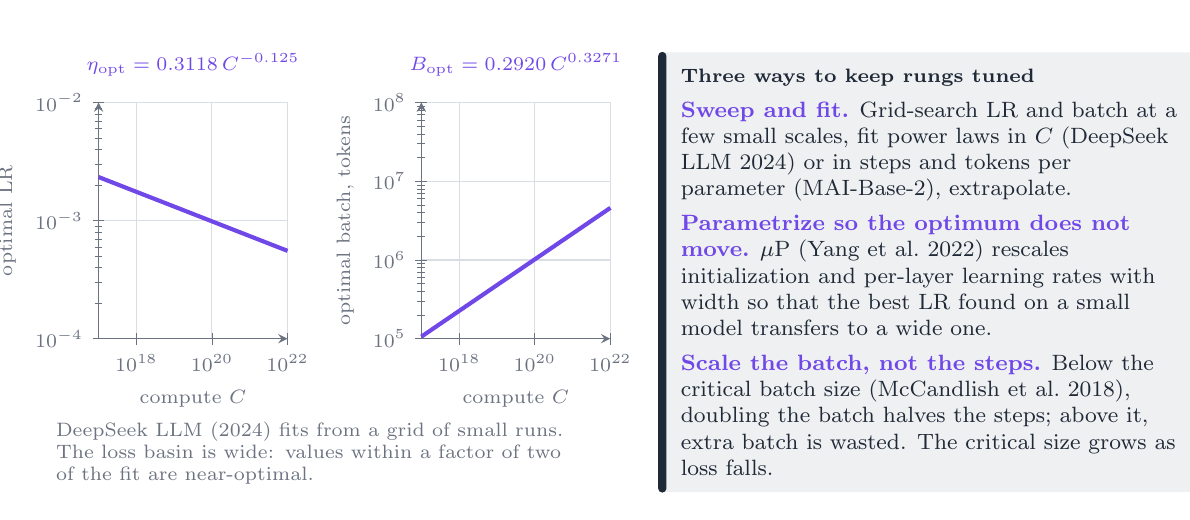
\begin{tikzpicture}
  \useasboundingbox (0,0) rectangle (14.4,5.9);
  \begin{axis}[lecture,at={(0.9cm,1.95cm)},anchor=south west,scale only axis,width=2.4cm,height=3.0cm,
      xmode=log,ymode=log,xmin=1e17,xmax=1e22,ymin=1e-4,ymax=1e-2,domain=1e17:1e22,samples=20,
      xlabel={compute $C$},ylabel={optimal LR},xtick={1e18,1e20,1e22},
      title={\scriptsize $\eta_{\text{opt}}=0.3118\,C^{-0.125}$},title style={text=posc}]
    \addplot[posc,line width=1.5pt] {0.3118*x^(-0.125)};
  \end{axis}
  \begin{axis}[lecture,at={(5.0cm,1.95cm)},anchor=south west,scale only axis,width=2.4cm,height=3.0cm,
      xmode=log,ymode=log,xmin=1e17,xmax=1e22,ymin=1e5,ymax=1e8,domain=1e17:1e22,samples=20,
      xlabel={compute $C$},ylabel={optimal batch, tokens},xtick={1e18,1e20,1e22},
      title={\scriptsize $B_{\text{opt}}=0.2920\,C^{0.3271}$},title style={text=posc}]
    \addplot[posc,line width=1.5pt] {0.2920*x^(0.3271)};
  \end{axis}
  \node[lab,anchor=north west,text width=6.6cm] at (0.3,0.95) {DeepSeek LLM (2024) fits from a grid of small runs. The loss basin is wide: values within a factor of two of the fit are near-optimal.};
  \bgpanel{8.0}{5.6}{6.3cm}{Three ways to keep rungs tuned}{%
    \hl{posc}{Sweep and fit.} Grid-search LR and batch at a few small scales,
    fit power laws in $C$ (DeepSeek LLM 2024) or in steps and tokens per
    parameter (MAI-Base-2), extrapolate.\\[3pt]
    \hl{posc}{Parametrize so the optimum does not move.} $\mu$P (Yang et al.\
    2022) rescales initialization and per-layer learning rates with width so
    that the best LR found on a small model transfers to a wide one.\\[3pt]
    \hl{posc}{Scale the batch, not the steps.} Below the critical batch size
    (McCandlish et al.\ 2018), doubling the batch halves the steps; above it,
    extra batch is wasted. The critical size grows as loss falls.}
\end{tikzpicture}
\end{frame}

% ---------------------------------------------------------------- 17
\begin{frame}{Refinement IV: the schedule decides what a point is worth}
\framesubtitle{Loss at the end of a cosine run is not the loss at the same token count inside a longer run. Ladders must control for it.}
\centering
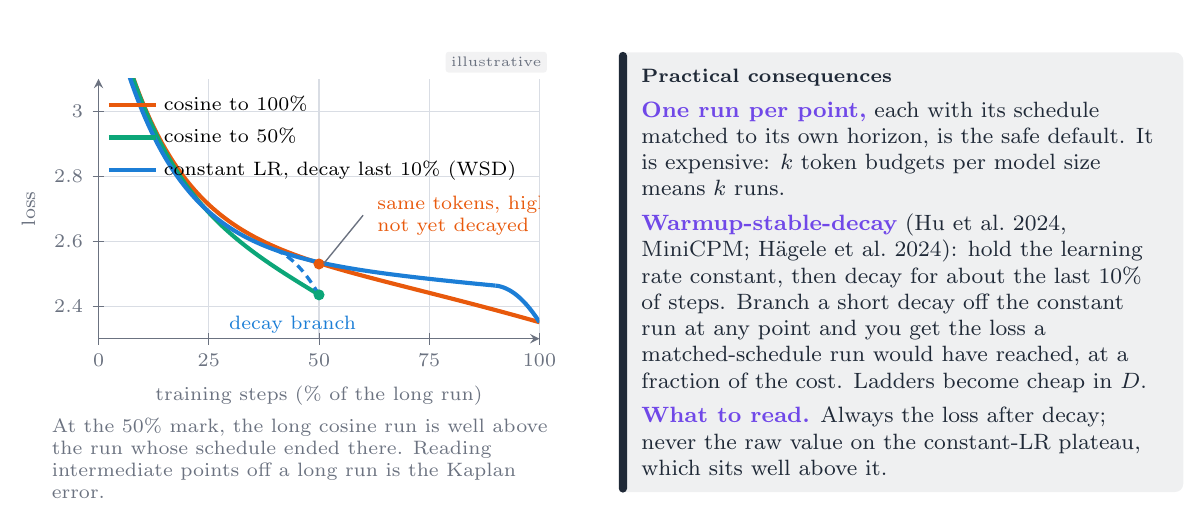
\begin{tikzpicture}
  \useasboundingbox (0,0) rectangle (14.4,5.9);
  \begin{axis}[lecture,at={(0.9cm,1.95cm)},anchor=south west,scale only axis,width=5.6cm,height=3.3cm,
      xmin=0,xmax=100,ymin=2.3,ymax=3.1,samples=120,clip=true,
      xlabel={training steps (\% of the long run)},ylabel={loss},
      legend style={at={(0.98,0.98)},anchor=north east},xtick={0,25,50,75,100},ytick={2.4,2.6,2.8,3.0}]
    \addplot[attn,line width=1.5pt,domain=0:100] {2.45+0.9*exp(-x/14)+0.12*(1-x/100)+0.03-0.13*(x/100)^2}; \addlegendentry{cosine to 100\%}
    \addplot[emb,line width=1.5pt,domain=0:50] {2.45+0.9*exp(-x/14)+0.12*(1-x/100)+0.03-0.13*(x/50)^2}; \addlegendentry{cosine to 50\%}
    \addplot[mlp,line width=1.5pt,domain=0:90] {2.45+0.9*exp(-x/14)+0.12*(1-x/100)}; \addlegendentry{constant LR, decay last 10\% (WSD)}
    \addplot[mlp,line width=1.5pt,domain=90:100] {2.45+0.9*exp(-x/14)+0.12*(1-x/100)-0.10*((x-90)/10)^2};
    \addplot[mlp,line width=1.2pt,densely dashed,domain=40:50] {2.45+0.9*exp(-x/14)+0.12*(1-x/100)-0.10*((x-40)/10)^2};
    \fill[attn] (axis cs:50,2.53) circle (2pt);
    \fill[emb] (axis cs:50,2.435) circle (2pt);
    \draw[muted,line width=0.5pt] (axis cs:51,2.53) -- (axis cs:60,2.68);
    \node[font=\scriptsize,text=attn,anchor=west,align=left] at (axis cs:61,2.68) {same tokens, higher loss:\\not yet decayed};
    \node[font=\scriptsize,text=mlp,anchor=north,align=center] at (axis cs:44,2.40) {decay branch};
  \end{axis}
  \srctag{6.6}{5.6}{illustrative}
  \node[txt,anchor=north west,text width=6.3cm,font=\scriptsize,text=muted] at (0.3,0.95)
    {At the 50\% mark, the long cosine run is well above the run whose schedule ended there. Reading intermediate points off a long run is the Kaplan error.};
  \bgpanel{7.5}{5.6}{6.6cm}{Practical consequences}{%
    \hl{posc}{One run per point,} each with its schedule matched to its own
    horizon, is the safe default. It is expensive: $k$ token budgets per model
    size means $k$ runs.\\[3pt]
    \hl{posc}{Warmup-stable-decay} (Hu et al.\ 2024, MiniCPM; Hägele et al.\
    2024): hold the learning rate constant, then decay for about the last
    10\% of steps. Branch a short decay off the constant run at any point and
    you get the loss a matched-schedule run would have reached, at a fraction
    of the cost. Ladders become cheap in $D$.\\[3pt]
    \hl{posc}{What to read.} Always the loss after decay; never the raw value
    on the constant-LR plateau, which sits well above it.}
\end{tikzpicture}
\end{frame}

% ---------------------------------------------------------------- 18
\begin{frame}{Refinement V: laws for architecture knobs}
\framesubtitle{Once the recipe is fixed, the same machinery answers narrower questions: how sparse, what vocabulary, what precision.}
\centering
\begin{tikzpicture}
  \useasboundingbox (0,0) rectangle (14.4,5.9);
  \foreach \x/\c/\ttl/\body/\who in {
      0.1/attn/{Mixture of experts}/{Loss follows a joint law in dense size and expert count. The gain over a dense model at equal active parameters shrinks slowly with scale but stays large; finer experts push the frontier further.}/{Clark et al.\ 2022; Krajewski et al.\ 2024},
      4.85/kct/{Vocabulary size}/{Vocabulary parameters scale differently from the rest. The optimal vocabulary grows with compute, more slowly than $N$; most models' vocabularies are smaller than the fit recommends.}/{Tao et al.\ 2024},
      9.6/trn/{Precision}/{Lower precision acts like fewer effective parameters, $N_{\text{eff}}=N\,f(P)$; post-training quantization hurts more the longer a model trained. Their fit puts compute-optimal precision near 7--8 bits.}/{Kumar et al.\ 2024}}{
    \node[anchor=north west,inner sep=0] at (\x,5.6) {%
      \begin{tikzpicture}
        \node[anchor=north west,minimum width=4.6cm,minimum height=3.85cm,rounded corners=4pt,fill=\c!8] (b) {};
        \fill[\c,rounded corners=2pt] (b.north west) rectangle ([yshift=-0.14cm]b.north east);
        \node[anchor=north west,text width=4.1cm,font=\small\bfseries,text=\c!85!black,inner sep=0] at ([xshift=8pt,yshift=-12pt]b.north west) {\ttl};
        \node[anchor=north west,text width=4.1cm,font=\scriptsize,text=ink,inner sep=0,align=flush left] at ([xshift=8pt,yshift=-30pt]b.north west) {\body};
        \node[anchor=south west,text width=4.1cm,font=\scriptsize,text=\c!85!black,inner sep=0] at ([xshift=8pt,yshift=7pt]b.south west) {\who};
      \end{tikzpicture}};}
  \node[txt,anchor=north west,text width=14.1cm] at (0.1,1.55) {%
    \hl{posc}{Data mixtures} (Ye et al.\ 2024): loss on each domain is a
    predictable function of the mixture proportions, so the mix can be chosen
    from small runs. \hl{posc}{The common pattern:} fix everything else, vary one
    knob across a few scales, fit a law with the knob as an extra variable, and
    extrapolate. Each such law is only trustworthy inside the recipe it was fit
    on.};
\end{tikzpicture}
\end{frame}

% ---------------------------------------------------------------- 19
\stage{6}
\begin{frame}{From loss to capability: what scaling laws do not promise}
\framesubtitle{Loss is smooth. A benchmark score is a nonlinear, often thresholded, function of it, and that is where ``emergence'' lives.}
\centering
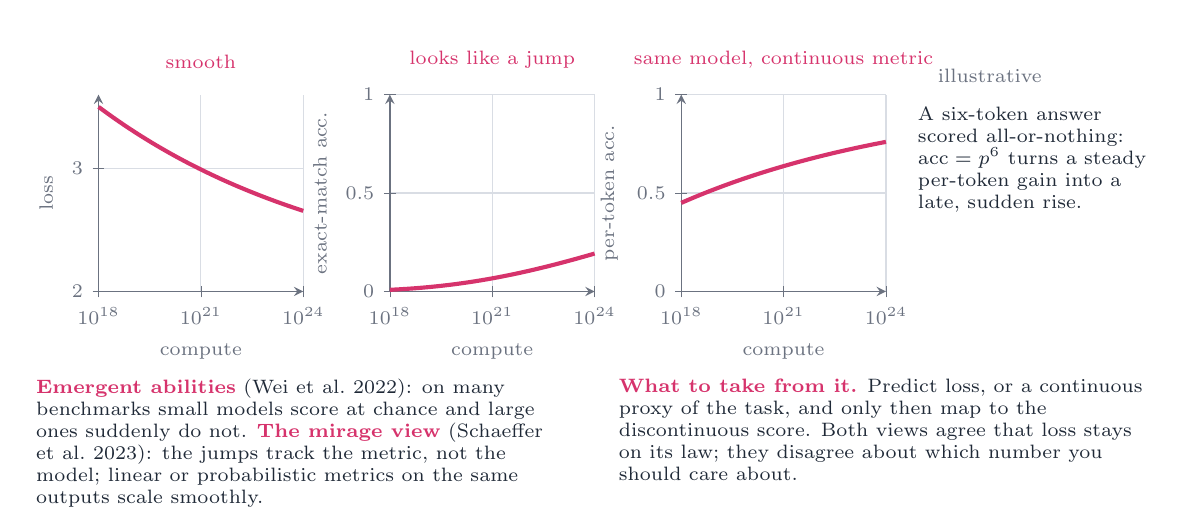
\begin{tikzpicture}
  \useasboundingbox (0,0) rectangle (14.4,5.9);
  \begin{axis}[lecture,at={(0.9cm,2.55cm)},anchor=south west,scale only axis,width=2.6cm,height=2.5cm,
      xmode=log,xmin=1e18,xmax=1e24,ymin=2.0,ymax=3.6,domain=1e18:1e24,samples=40,
      xlabel={compute},ylabel={loss},xtick={1e18,1e21,1e24},ytick={2,3},title={\scriptsize smooth},title style={text=outc}]
    \addplot[outc,line width=1.5pt] {2.0+1.5*(x/1e18)^(-0.06)};
  \end{axis}
  \begin{axis}[lecture,at={(4.6cm,2.55cm)},anchor=south west,scale only axis,width=2.6cm,height=2.5cm,
      xmode=log,xmin=1e18,xmax=1e24,ymin=0,ymax=1,domain=1e18:1e24,samples=60,
      xlabel={compute},ylabel={exact-match acc.},xtick={1e18,1e21,1e24},ytick={0,0.5,1},title={\scriptsize looks like a jump},title style={text=outc}]
    \addplot[outc,line width=1.5pt] {(0.45+0.55*(1-(x/1e18)^(-0.06)))^6};
  \end{axis}
  \begin{axis}[lecture,at={(8.3cm,2.55cm)},anchor=south west,scale only axis,width=2.6cm,height=2.5cm,
      xmode=log,xmin=1e18,xmax=1e24,ymin=0,ymax=1,domain=1e18:1e24,samples=60,
      xlabel={compute},ylabel={per-token acc.},xtick={1e18,1e21,1e24},ytick={0,0.5,1},title={\scriptsize same model, continuous metric},title style={text=outc}]
    \addplot[outc,line width=1.5pt] {0.45+0.55*(1-(x/1e18)^(-0.06))};
  \end{axis}
  \node[lab,anchor=south west] at (11.5,5.15) {illustrative};
  \node[txt,anchor=north west,text width=2.9cm,font=\scriptsize] at (11.3,4.9) {%
    A six-token answer scored all-or-nothing: $\text{acc}=p^6$ turns a steady
    per-token gain into a late, sudden rise.};
  \node[txt,anchor=north west,text width=6.7cm,font=\scriptsize] at (0.1,1.45) {%
    \hl{outc}{Emergent abilities} (Wei et al.\ 2022): on many benchmarks small
    models score at chance and large ones suddenly do not. \hl{outc}{The
    mirage view} (Schaeffer et al.\ 2023): the jumps track the metric, not the
    model; linear or probabilistic metrics on the same outputs scale smoothly.};
  \node[txt,anchor=north west,text width=6.7cm,font=\scriptsize] at (7.5,1.45) {%
    \hl{outc}{What to take from it.} Predict loss, or a continuous proxy of the
    task, and only then map to the discontinuous score. Both views agree that
    loss stays on its law; they disagree about which number you should care
    about.};
\end{tikzpicture}
\end{frame}

% ---------------------------------------------------------------- 20
\begin{frame}{Predicting a benchmark score: the two-stage map}
\framesubtitle{Fit compute to a continuous intermediate quantity, then that quantity to the score. Each stage is better behaved than the whole.}
\centering
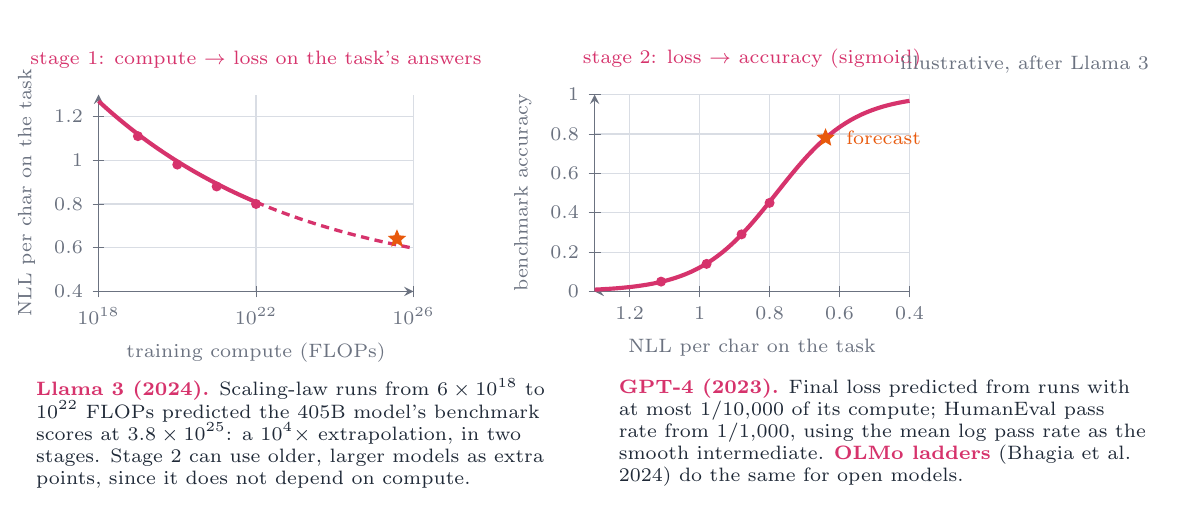
\begin{tikzpicture}
  \useasboundingbox (0,0) rectangle (14.4,5.9);
  \begin{axis}[lecture,at={(0.9cm,2.55cm)},anchor=south west,scale only axis,width=4.0cm,height=2.5cm,
      xmode=log,xmin=1e18,xmax=1e26,ymin=0.4,ymax=1.3,domain=1e18:1e26,samples=40,
      xlabel={training compute (FLOPs)},ylabel={NLL per char on the task},xtick={1e18,1e22,1e26},
      title={\scriptsize stage 1: compute $\to$ loss on the task's answers},title style={text=outc}]
    \addplot[outc,line width=1.5pt,domain=1e18:1e22] {0.42+0.85*(x/1e18)^(-0.085)};
    \addplot[outc,line width=1.2pt,densely dashed,domain=1e22:1e26] {0.42+0.85*(x/1e18)^(-0.085)};
    \addplot[only marks,mark=*,mark size=1.6pt,outc] coordinates {(1e19,1.11)(1e20,0.98)(1e21,0.88)(1e22,0.80)};
    \node[star,star points=5,star point ratio=2.2,fill=attn,inner sep=0pt,minimum size=7pt] at (axis cs:3.8e25,0.64) {};
  \end{axis}
  \begin{axis}[lecture,at={(7.2cm,2.55cm)},anchor=south west,scale only axis,width=4.0cm,height=2.5cm,
      xmin=0.4,xmax=1.3,ymin=0,ymax=1,domain=0.4:1.3,samples=60,x dir=reverse,
      xlabel={NLL per char on the task},ylabel={benchmark accuracy},
      title={\scriptsize stage 2: loss $\to$ accuracy (sigmoid)},title style={text=outc}]
    \addplot[outc,line width=1.5pt] {1/(1+exp(9*(x-0.78)))};
    \addplot[only marks,mark=*,mark size=1.6pt,outc] coordinates {(1.11,0.05)(0.98,0.14)(0.88,0.29)(0.80,0.45)};
    \node[star,star points=5,star point ratio=2.2,fill=attn,inner sep=0pt,minimum size=7pt] at (axis cs:0.64,0.78) {};
    \node[font=\scriptsize,text=attn,anchor=west] at (axis cs:0.63,0.78) {\ forecast};
  \end{axis}
  \node[lab,anchor=north east] at (14.3,5.6) {illustrative, after Llama 3};
  \node[txt,anchor=north west,text width=6.7cm,font=\scriptsize] at (0.1,1.45) {%
    \hl{outc}{Llama 3 (2024).} Scaling-law runs from $6\times10^{18}$ to
    $10^{22}$ FLOPs predicted the 405B model's benchmark scores at
    $3.8\times10^{25}$: a $10^4\times$ extrapolation, in two stages. Stage 2 can
    use older, larger models as extra points, since it does not depend on compute.};
  \node[txt,anchor=north west,text width=6.7cm,font=\scriptsize] at (7.5,1.45) {%
    \hl{outc}{GPT-4 (2023).} Final loss predicted from runs with at most
    $1/10{,}000$ of its compute; HumanEval pass rate from $1/1{,}000$, using the
    mean log pass rate as the smooth intermediate. \hl{outc}{OLMo ladders}
    (Bhagia et al.\ 2024) do the same for open models.};
\end{tikzpicture}
\end{frame}

% ---------------------------------------------------------------- 21
\stage{7}
\begin{frame}{The ladder: one recipe, several sizes, one fit}
\framesubtitle{A scaling ladder is a set of models that differ only in scale. Everything else is held fixed so that scale is the only variable.}
\centering
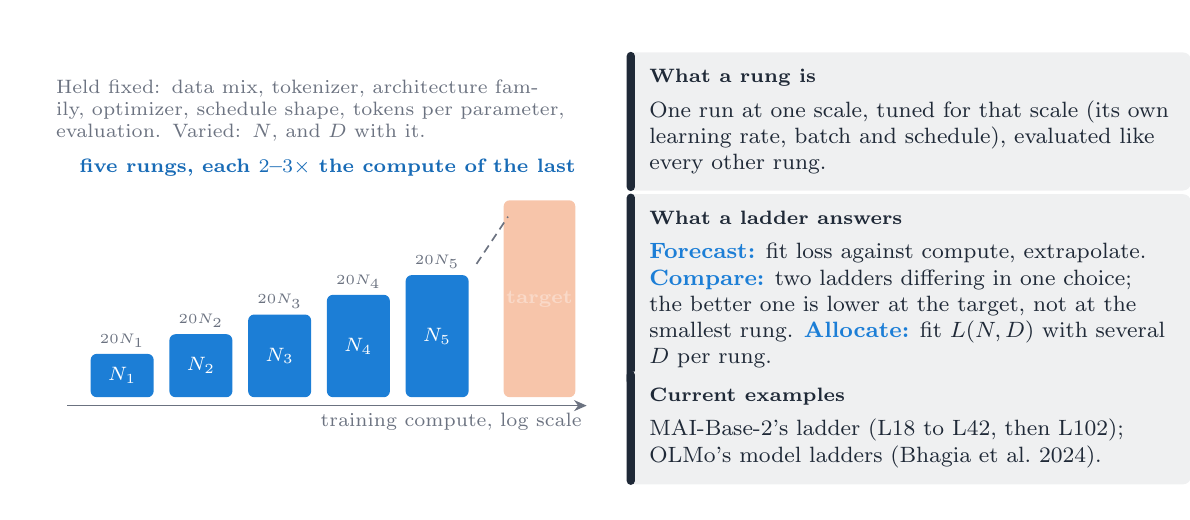
\begin{tikzpicture}
  \useasboundingbox (0,0) rectangle (14.4,5.9);
  % ladder sketch
  \draw[muted,line width=0.6pt,->] (0.5,1.1) -- (7.1,1.1) node[below left,lab,yshift=-1pt]{training compute, log scale};
  \foreach \k/\x/\h/\lab/\tok in {1/1.2/0.55/{$N_1$}/{$20N_1$},2/2.2/0.8/{$N_2$}/{$20N_2$},3/3.2/1.05/{$N_3$}/{$20N_3$},4/4.2/1.3/{$N_4$}/{$20N_4$},5/5.2/1.55/{$N_5$}/{$20N_5$}}{
    \node[fillbox=mlp,minimum width=0.8cm,minimum height=\h cm,inner sep=1pt,font=\scriptsize\bfseries,anchor=south] at (\x,1.2) {\lab};
    \node[lab,anchor=south,font=\tiny] at (\x,{1.2+\h+0.03}) {\tok};}
  \node[lab,anchor=south west,text=mlp!85!black,font=\scriptsize\bfseries] at (0.6,3.95) {five rungs, each $2$--$3\times$ the compute of the last};
  \node[fillbox=attn,minimum width=0.8cm,minimum height=2.5cm,inner sep=1pt,font=\scriptsize\bfseries,anchor=south,opacity=0.35] at (6.5,1.2) {target};
  \draw[muted,densely dashed,line width=0.6pt] (5.7,2.9) -- (6.1,3.5);
  \node[lab,anchor=north west,text width=6.6cm] at (0.3,5.3) {Held fixed: data mix, tokenizer, architecture family, optimizer, schedule shape, tokens per parameter, evaluation. Varied: $N$, and $D$ with it.};
  \bgpanel{7.6}{5.6}{6.6cm}{What a rung is}{%
    One run at one scale, tuned for that scale (its own learning rate, batch
    and schedule), evaluated like every other rung.}
  \bgpanel{7.6}{3.8}{6.6cm}{What a ladder answers}{%
    \hl{mlp}{Forecast:} fit loss against compute, extrapolate.
    \hl{mlp}{Compare:} two ladders differing in one choice; the better one is
    lower at the target, not at the smallest rung. \hl{mlp}{Allocate:} fit
    $L(N,D)$ with several $D$ per rung.}
  \bgpanel{7.6}{1.55}{6.6cm}{Current examples}{%
    MAI-Base-2's ladder (L18 to L42, then L102); OLMo's model ladders
    (Bhagia et al.\ 2024).}
\end{tikzpicture}
\end{frame}

% ---------------------------------------------------------------- 22
\begin{frame}{Designing a ladder: the choices and the usual answers}
\framesubtitle{A ladder is an experiment. Decide what is fixed, what is varied, how many points, and what is measured, before any run starts.}
\centering
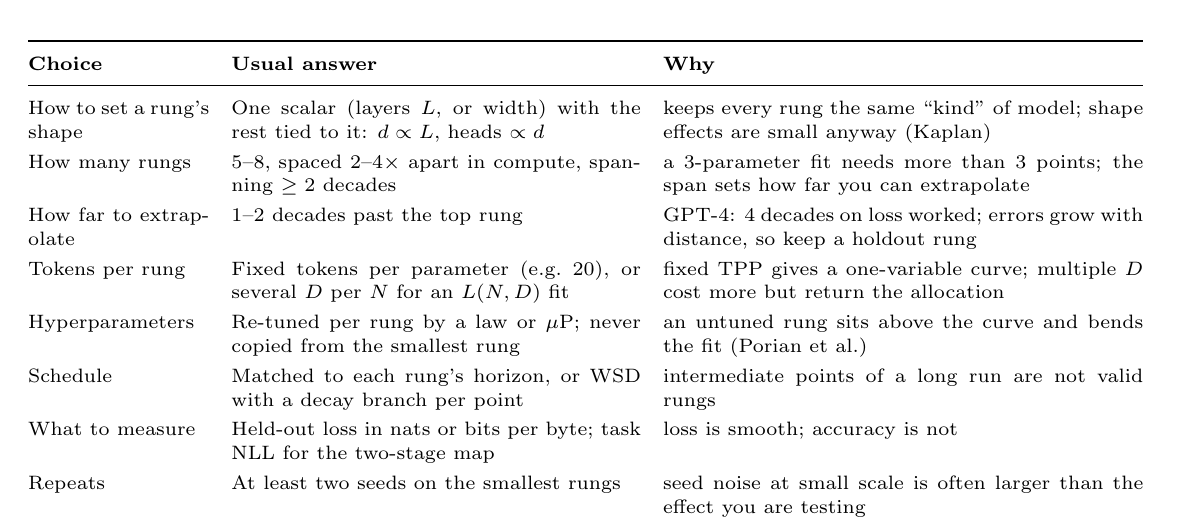
\begin{tikzpicture}
  \useasboundingbox (0,0) rectangle (14.4,5.9);
  \node[anchor=north west,inner sep=0,font=\fontsize{6.8}{8.6}\selectfont] at (0.0,5.75) {%
    \renewcommand{\arraystretch}{1.25}\setlength{\tabcolsep}{4pt}%
    \begin{tabular}{@{}p{2.3cm}p{5.2cm}p{6.1cm}@{}}
      \toprule
      \textbf{Choice} & \textbf{Usual answer} & \textbf{Why}\\
      \midrule
      How to set a rung's shape & One scalar (layers $L$, or width) with the rest tied to it: $d\propto L$, heads $\propto d$ & keeps every rung the same ``kind'' of model; shape effects are small anyway (Kaplan)\\
      How many rungs & 5--8, spaced $2$--$4\times$ apart in compute, spanning $\ge2$ decades & a 3-parameter fit needs more than 3 points; the span sets how far you can extrapolate\\
      How far to extrapolate & 1--2 decades past the top rung & GPT-4: 4 decades on loss worked; errors grow with distance, so keep a holdout rung\\
      Tokens per rung & Fixed tokens per parameter (e.g.\ 20), or several $D$ per $N$ for an $L(N,D)$ fit & fixed TPP gives a one-variable curve; multiple $D$ cost more but return the allocation\\
      Hyperparameters & Re-tuned per rung by a law or $\mu$P; never copied from the smallest rung & an untuned rung sits above the curve and bends the fit (Porian et al.)\\
      Schedule & Matched to each rung's horizon, or WSD with a decay branch per point & intermediate points of a long run are not valid rungs\\
      What to measure & Held-out loss in nats or bits per byte; task NLL for the two-stage map & loss is smooth; accuracy is not\\
      Repeats & At least two seeds on the smallest rungs & seed noise at small scale is often larger than the effect you are testing\\
      \bottomrule
    \end{tabular}};
\end{tikzpicture}
\end{frame}

% ---------------------------------------------------------------- 23
\begin{frame}{Fitting the law and reading the forecast}
\framesubtitle{Fit in log space, hold out the top rung, report the spread. A forecast without an error bar is a guess with a decimal point.}
\centering
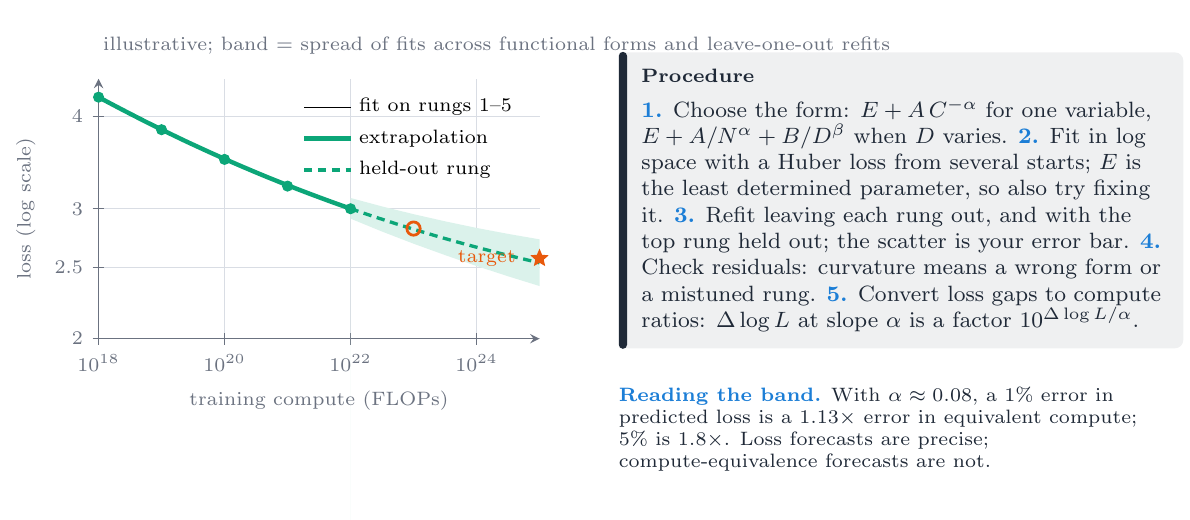
\begin{tikzpicture}
  \useasboundingbox (0,0) rectangle (14.4,5.9);
  \begin{axis}[lecture,at={(0.9cm,1.95cm)},anchor=south west,scale only axis,width=5.6cm,height=3.3cm,
      xmode=log,ymode=log,xmin=1e18,xmax=1e25,ymin=2.0,ymax=4.5,domain=1e18:1e25,samples=50,
      xlabel={training compute (FLOPs)},ylabel={loss (log scale)},
      ytick={2,2.5,3,4},yticklabels={2,2.5,3,4},xtick={1e18,1e20,1e22,1e24},legend pos=north east]
    \addplot[draw=none,fill=emb!15] coordinates {(1.000e+22,3.103) (3.162e+22,3.022) (1.000e+23,2.950) (3.162e+23,2.885) (1.000e+24,2.826) (3.162e+24,2.774) (1.000e+25,2.727) (1.000e+25,2.357) (3.162e+24,2.430) (1.000e+24,2.509) (3.162e+23,2.596) (1.000e+23,2.690) (3.162e+22,2.794) (1.000e+22,2.909)} \closedcycle;
    \addplot[emb,line width=1.6pt,domain=1e18:1e22] {1.95+2.3*(x/1e18)^(-0.085)}; \addlegendentry{fit on rungs 1--5}
    \addplot[emb,line width=1.2pt,densely dashed,domain=1e22:1e25] {1.95+2.3*(x/1e18)^(-0.085)}; \addlegendentry{extrapolation}
    \addplot[only marks,mark=*,mark size=1.8pt,emb] coordinates {(1e18,4.25)(1e19,3.84)(1e20,3.5)(1e21,3.22)(1e22,3.0)};
    \addplot[only marks,mark=o,mark size=2.4pt,line width=1pt,attn] coordinates {(1e23,2.82)}; \addlegendentry{held-out rung}
    \node[star,star points=5,star point ratio=2.2,fill=attn,inner sep=0pt,minimum size=7pt] at (axis cs:1e25,2.57) {};
    \node[font=\scriptsize,text=attn,anchor=east] at (axis cs:6e24,2.57) {target};
  \end{axis}
  \node[lab,anchor=south west] at (0.9,5.5) {illustrative; band = spread of fits across functional forms and leave-one-out refits};
  \bgpanel{7.5}{5.6}{6.6cm}{Procedure}{%
    \hl{mlp}{1.} Choose the form: $E+A\,C^{-\alpha}$ for one variable,
    $E+A/N^{\alpha}+B/D^{\beta}$ when $D$ varies. \hl{mlp}{2.} Fit in log
    space with a Huber loss from several starts; $E$ is the least determined
    parameter, so also try fixing it. \hl{mlp}{3.} Refit leaving each rung
    out, and with the top rung held out; the scatter is your error bar.
    \hl{mlp}{4.} Check residuals: curvature means a wrong form or a mistuned
    rung. \hl{mlp}{5.} Convert loss gaps to compute ratios:
    $\Delta\log L$ at slope $\alpha$ is a factor $10^{\Delta\log L/\alpha}$.}
  \node[txt,anchor=north west,text width=6.6cm,font=\scriptsize] at (7.5,1.35) {%
    \hl{mlp}{Reading the band.} With $\alpha\approx0.08$, a 1\% error in
    predicted loss is a $1.13\times$ error in equivalent compute; 5\% is
    $1.8\times$. Loss forecasts are precise; compute-equivalence forecasts are
    not.};
\end{tikzpicture}
\end{frame}

% ---------------------------------------------------------------- 24
\stage{8}
\begin{frame}{Worked example: a \$1M scaling study}
\framesubtitle{Fictional but realistic numbers. Convert dollars to FLOPs, choose the rungs, decide what each can and cannot tell you.}
\centering
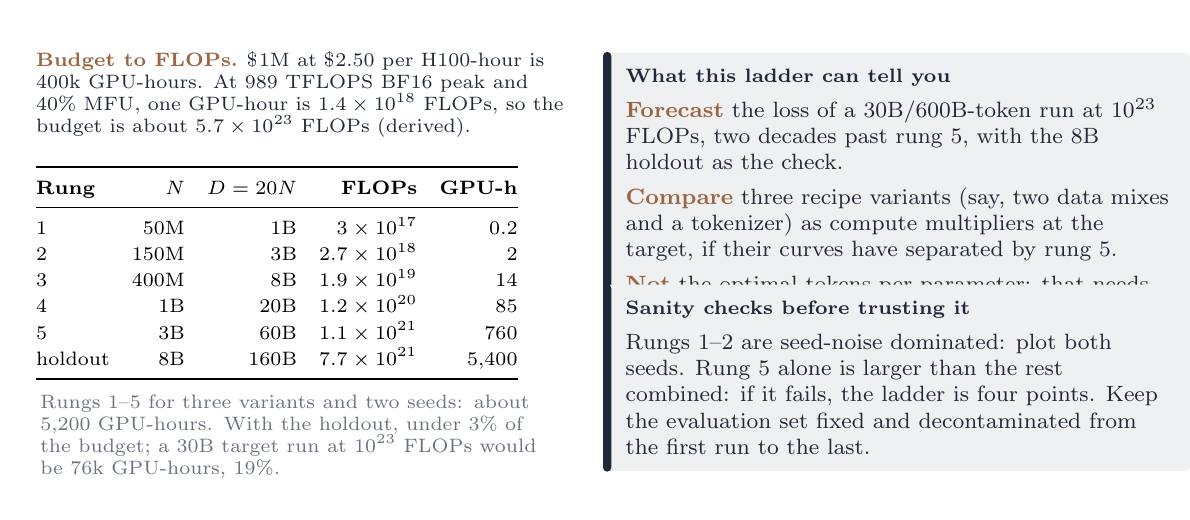
\begin{tikzpicture}
  \useasboundingbox (0,0) rectangle (14.4,5.9);
  \node[txt,anchor=north west,text width=6.7cm,font=\scriptsize] at (0.1,5.6) {%
    \hl{trn}{Budget to FLOPs.} \$1M at \$2.50 per H100-hour is 400k GPU-hours.
    At 989 TFLOPS BF16 peak and 40\% MFU, one GPU-hour is $1.4\times10^{18}$
    FLOPs, so the budget is about $5.7\times10^{23}$ FLOPs (derived).};
  \node[anchor=north west,inner sep=0,font=\fontsize{6.8}{8.6}\selectfont] at (0.1,4.15) {%
    \renewcommand{\arraystretch}{1.1}\setlength{\tabcolsep}{4pt}%
    \begin{tabular}{@{}lrrrr@{}}
      \toprule
      \textbf{Rung} & \textbf{$N$} & \textbf{$D=20N$} & \textbf{FLOPs} & \textbf{GPU-h}\\
      \midrule
      1 & 50M  & 1B   & $3\times10^{17}$   & 0.2\\
      2 & 150M & 3B   & $2.7\times10^{18}$ & 2\\
      3 & 400M & 8B   & $1.9\times10^{19}$ & 14\\
      4 & 1B   & 20B  & $1.2\times10^{20}$ & 85\\
      5 & 3B   & 60B  & $1.1\times10^{21}$ & 760\\
      holdout & 8B & 160B & $7.7\times10^{21}$ & 5{,}400\\
      \bottomrule
    \end{tabular}};
  \node[lab,anchor=north west,text width=6.6cm] at (0.1,1.3) {Rungs 1--5 for three variants and two seeds: about 5{,}200 GPU-hours. With the holdout, under 3\% of the budget; a 30B target run at $10^{23}$ FLOPs would be 76k GPU-hours, 19\%.};
  \bgpanel{7.3}{5.6}{6.9cm}{What this ladder can tell you}{%
    \hl{trn}{Forecast} the loss of a 30B/600B-token run at $10^{23}$ FLOPs,
    two decades past rung 5, with the 8B holdout as the check.\\[3pt]
    \hl{trn}{Compare} three recipe variants (say, two data mixes and a
    tokenizer) as compute multipliers at the target, if their curves have
    separated by rung 5.\\[3pt]
    \hl{trn}{Not} the optimal tokens per parameter: that needs several $D$ per
    rung, roughly tripling the ladder cost.}
  \bgpanel{7.3}{2.65}{6.9cm}{Sanity checks before trusting it}{%
    Rungs 1--2 are seed-noise dominated: plot both seeds. Rung 5 alone is
    larger than the rest combined: if it fails, the ladder is four points. Keep
    the evaluation set fixed and decontaminated from the first run to the last.}
\end{tikzpicture}
\end{frame}

% ---------------------------------------------------------------- 25
\begin{frame}{Pitfalls: how scaling experiments go wrong}
\framesubtitle{Most failed forecasts trace back to one of these. Each has shown up in a published paper at least once.}
\centering
\begin{tikzpicture}
  \useasboundingbox (0,0) rectangle (14.4,5.9);
  \foreach \x/\y/\num/\ttl/\body in {
      0.1/5.6/1/{Points off one long run}/{Intermediate losses of a cosine run overstate what a matched-horizon run would reach. Use one run per point or a WSD branch.},
      4.85/5.6/2/{Copying hyperparameters up}/{The best LR shrinks and the best batch grows with scale. An untuned rung sits above the curve and tilts the fit.},
      9.6/5.6/3/{Extrapolating too far}/{Two decades past the top rung is routine; four worked for GPT-4 on loss. Keep a holdout rung and report the spread of refits.},
      0.1/3.45/4/{Comparing at the wrong scale}/{Recipe A beats B at 50M and loses at 3B. Compare curves at the target, and only call it when the curves have separated beyond seed noise.},
      4.85/3.45/5/{Changing two things at once}/{A new tokenizer changes the loss unit (nats per token); compare in bits per byte, and change one variable per ladder.},
      9.6/3.45/6/{Trusting the floor}/{$E$ is the least determined constant and dominates long extrapolations. Fit with and without it; if forecasts diverge, you need a higher rung.}}{
    \node[anchor=north west,inner sep=0] at (\x,\y) {%
      \begin{tikzpicture}
        \node[anchor=north west,text width=4.15cm,align=flush left,font=\scriptsize,text=ink,minimum height=2.0cm,
              inner xsep=6pt,inner ysep=5pt,rounded corners=3pt,fill=trn!8] (c)
              {{\color{trn}\bfseries\num\ \ \ttl}\\[2pt]\body};
      \end{tikzpicture}};}
  \node[txt,anchor=north west,text width=14.1cm,font=\scriptsize] at (0.1,1.2) {%
    \hl{trn}{Also:} evaluation sets contaminated by training data (the floor
    looks lower than it is); loss measured on a different distribution than the
    one the law was fit on; embedding parameters counted inconsistently across
    rungs; and mixing runs with different precision or numerics.};
\end{tikzpicture}
\end{frame}

% ---------------------------------------------------------------- 26
\stage{9}
\begin{frame}{The frontier: where the laws are being pushed}
\framesubtitle{The 2020--22 picture still holds for dense pretraining. Four developments change what is on the axes.}
\centering
\begin{tikzpicture}
  \useasboundingbox (0,0) rectangle (14.4,5.9);
  \foreach \x/\y/\c/\ttl/\body in {
      0.1/5.6/attn/{Sparse models}/{Mixture-of-experts models separate parameters from compute per token. Laws now carry two sizes (total and active) and an expert count; MAI-Base-2 at 2.8T/80B is a current data point.},
      7.3/5.6/kct/{Data as the constraint}/{Public text is finite. Repetition laws (Muennighoff), synthetic data and curation become part of the recipe, and ladders must repeat data on every rung to stay honest.},
      0.1/3.4/vc/{Laws for the whole recipe}/{Learning rate, weight decay, dropout, vocabulary, precision and mixture each get a fitted law. The ladder is now a system that predicts the full configuration of the big run, not only its loss.},
      7.3/3.4/posc/{Beyond the pretraining loss}/{The loss floor and the two-stage map give a benchmark forecast. What they do not cover is post-training or compute spent at inference, which change capability without touching the pretraining law.}}{
    \node[anchor=north west,inner sep=0] at (\x,\y) {%
      \begin{tikzpicture}
        \node[anchor=north west,text width=6.5cm,align=flush left,font=\scriptsize,text=ink,minimum height=1.95cm,
              inner xsep=7pt,inner ysep=6pt,rounded corners=3pt,fill=\c!8] (c)
              {{\color{\c!85!black}\bfseries\small\ttl}\\[3pt]\body};
        \fill[\c,rounded corners=1.5pt] (c.north west) rectangle ([xshift=3pt]c.south west);
      \end{tikzpicture}};}
  \node[txt,anchor=north west,text width=14.1cm] at (0.1,1.1) {%
    \hl{vc}{The constant through all of it:} a straight line on log axes,
    measured on a ladder, extrapolated with an error bar. The axes change; the
    method does not.};
\end{tikzpicture}
\end{frame}

% ---------------------------------------------------------------- 27
\begin{frame}{Case study: the MAI-Base-2 ladder (2026)}
\framesubtitle{Everything in this lecture, applied once: five rungs over two decades, a forecast two decades out, and the forecast held.}
\centering
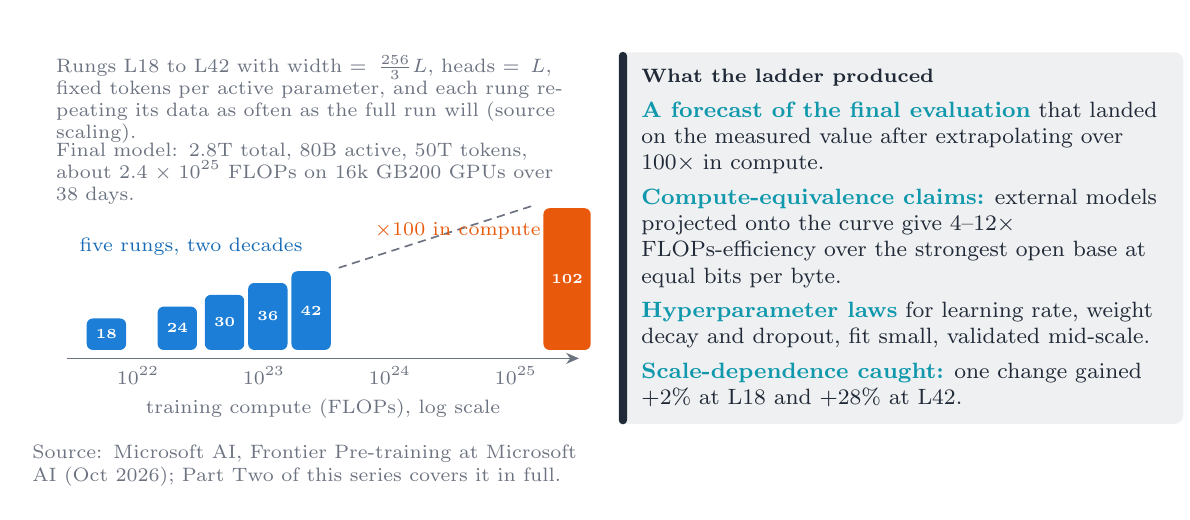
\begin{tikzpicture}
  \useasboundingbox (0,0) rectangle (14.4,5.9);
  \node[lab,anchor=north west,text width=6.7cm] at (0.3,5.6) {Rungs L18 to L42 with width $=\tfrac{256}{3}L$, heads $=L$, fixed tokens per active parameter, and each rung repeating its data as often as the full run will (source scaling).};
  \draw[muted,line width=0.6pt,->] (0.5,1.7) -- (7.0,1.7);
  \node[lab,anchor=north] at (3.75,1.25) {training compute (FLOPs), log scale};
  \foreach \e/\x in {22/1.4,23/3.0,24/4.6,25/6.2} \node[lab,anchor=north] at (\x,1.65) {$10^{\e}$};
  \foreach \L/\x/\h in {18/1.0/0.4,24/1.9/0.55,30/2.5/0.7,36/3.05/0.85,42/3.6/1.0}
    \node[fillbox=mlp,minimum width=0.5cm,minimum height=\h cm,inner sep=0pt,font=\tiny\bfseries,anchor=south] at (\x,1.8) {\L};
  \node[fillbox=attn,minimum width=0.6cm,minimum height=1.8cm,inner sep=0pt,font=\tiny\bfseries,anchor=south] at (6.85,1.8) {102};
  \draw[muted,densely dashed,line width=0.6pt] (3.95,2.85) -- (6.45,3.65);
  \node[lab,anchor=south west,text=attn] at (4.35,3.15) {$\times100$ in compute};
  \node[lab,anchor=south west,text=mlp!85!black] at (0.6,2.95) {five rungs, two decades};
  \node[lab,anchor=north west,text width=6.7cm] at (0.3,4.5) {Final model: 2.8T total, 80B active, 50T tokens, about $2.4\times10^{25}$ FLOPs on 16k GB200 GPUs over 38 days.};
  \bgpanel{7.5}{5.6}{6.6cm}{What the ladder produced}{%
    \hl{vc}{A forecast of the final evaluation} that landed on the measured
    value after extrapolating over $100\times$ in compute.\\[3pt]
    \hl{vc}{Compute-equivalence claims:} external models projected onto the
    curve give $4$--$12\times$ FLOPs-efficiency over the strongest open base
    at equal bits per byte.\\[3pt]
    \hl{vc}{Hyperparameter laws} for learning rate, weight decay and dropout,
    fit small, validated mid-scale.\\[3pt]
    \hl{vc}{Scale-dependence caught:} one change gained $+2\%$ at L18 and
    $+28\%$ at L42.}
  \node[lab,anchor=south west,text width=7.2cm] at (0.0,0.02) {Source: Microsoft AI, Frontier Pre-training at Microsoft AI (Oct 2026); Part Two of this series covers it in full.};
\end{tikzpicture}
\end{frame}

% ---------------------------------------------------------------- 28
\begin{frame}{Exercises}
\framesubtitle{Three short ones to do by hand, two that need a GPU. Answers to the first three are on the next slide.}
\centering
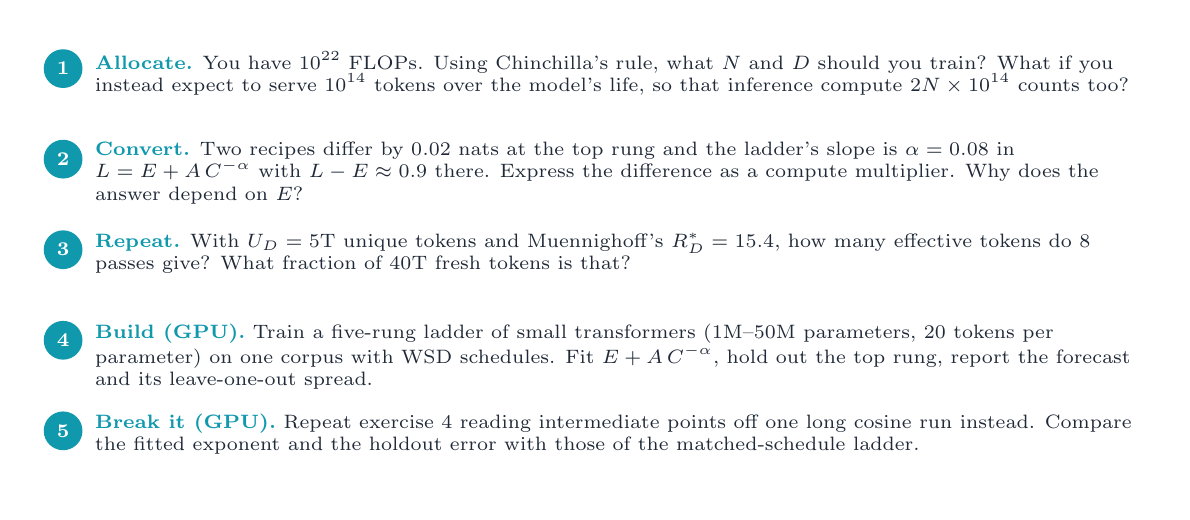
\begin{tikzpicture}
  \useasboundingbox (0,0) rectangle (14.4,5.9);
  \foreach \y/\num/\body in {
      5.6/1/{\hl{vc}{Allocate.} You have $10^{22}$ FLOPs. Using Chinchilla's rule, what $N$ and $D$ should you train? What if you instead expect to serve $10^{14}$ tokens over the model's life, so that inference compute $2N\times10^{14}$ counts too?},
      4.45/2/{\hl{vc}{Convert.} Two recipes differ by $0.02$ nats at the top rung and the ladder's slope is $\alpha=0.08$ in $L=E+A\,C^{-\alpha}$ with $L-E\approx0.9$ there. Express the difference as a compute multiplier. Why does the answer depend on $E$?},
      3.3/3/{\hl{vc}{Repeat.} With $U_D=5$T unique tokens and Muennighoff's $R_D^*=15.4$, how many effective tokens do 8 passes give? What fraction of 40T fresh tokens is that?},
      2.15/4/{\hl{vc}{Build (GPU).} Train a five-rung ladder of small transformers (1M--50M parameters, 20 tokens per parameter) on one corpus with WSD schedules. Fit $E+A\,C^{-\alpha}$, hold out the top rung, report the forecast and its leave-one-out spread.},
      1.0/5/{\hl{vc}{Break it (GPU).} Repeat exercise 4 reading intermediate points off one long cosine run instead. Compare the fitted exponent and the holdout error with those of the matched-schedule ladder.}}{
    \node[circle,fill=vc,text=white,font=\scriptsize\bfseries,inner sep=0pt,minimum size=14pt] at (0.45,\y-0.22) {\num};
    \node[txt,anchor=north west,text width=13.3cm,font=\scriptsize] at (0.85,\y) {\body};}
\end{tikzpicture}
\end{frame}

% ---------------------------------------------------------------- 29
\begin{frame}{Worked answers to exercises 1--3}
\framesubtitle{Showing the arithmetic, since the point of the lecture is that these are back-of-envelope calculations.}
\centering
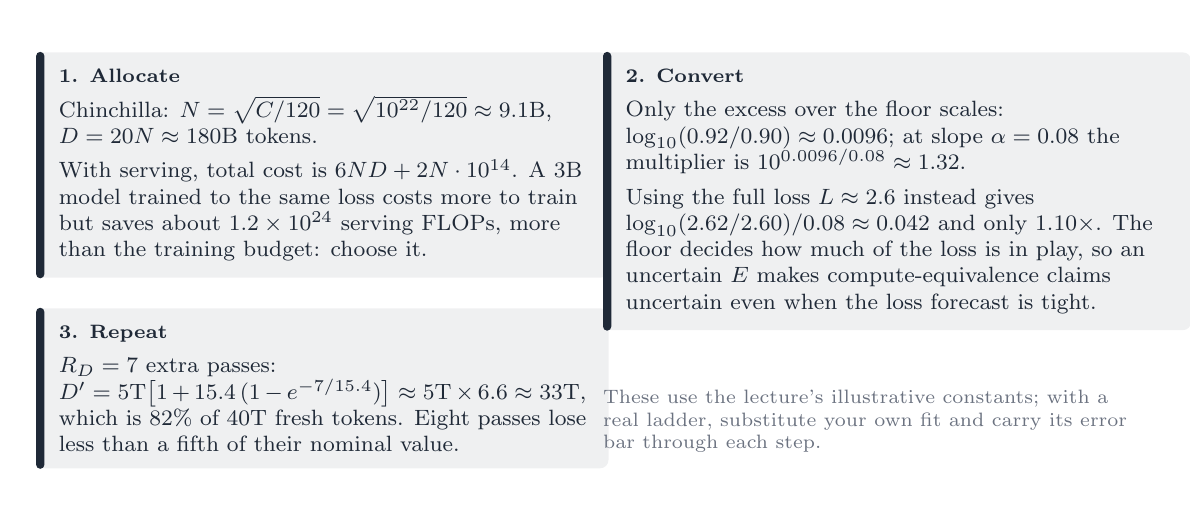
\begin{tikzpicture}
  \useasboundingbox (0,0) rectangle (14.4,5.9);
  \bgpanel{0.1}{5.6}{6.7cm}{1. Allocate}{%
    Chinchilla: $N=\sqrt{C/120}=\sqrt{10^{22}/120}\approx9.1\text{B}$,
    $D=20N\approx180\text{B}$ tokens.\\[3pt]
    With serving, total cost is $6ND+2N\cdot10^{14}$. A 3B model trained to
    the same loss costs more to train but saves about $1.2\times10^{24}$
    serving FLOPs, more than the training budget: choose it.}
  \bgpanel{0.1}{2.35}{6.7cm}{3. Repeat}{%
    $R_D=7$ extra passes: $D'=5\text{T}\big[1+15.4\,(1-e^{-7/15.4})\big]
    \approx5\text{T}\times6.6\approx33\text{T}$, which is 82\% of 40T fresh
    tokens. Eight passes lose less than a fifth of their nominal value.}
  \bgpanel{7.3}{5.6}{6.9cm}{2. Convert}{%
    Only the excess over the floor scales:
    $\log_{10}(0.92/0.90)\approx0.0096$; at slope $\alpha=0.08$ the
    multiplier is $10^{0.0096/0.08}\approx1.32$.\\[3pt]
    Using the full loss $L\approx2.6$ instead gives
    $\log_{10}(2.62/2.60)/0.08\approx0.042$ and only $1.10\times$. The floor
    decides how much of the loss is in play, so an uncertain $E$ makes
    compute-equivalence claims uncertain even when the loss forecast is tight.}
  \node[txt,anchor=north west,text width=6.9cm,font=\scriptsize,text=muted] at (7.3,1.3) {%
    These use the lecture's illustrative constants; with a real ladder, substitute
    your own fit and carry its error bar through each step.};
\end{tikzpicture}
\end{frame}

% ---------------------------------------------------------------- 30
\stage{10}
\begin{frame}{Summary: what to remember}
\framesubtitle{Six statements that survive every paper in this lecture.}
\centering
\begin{tikzpicture}
  \useasboundingbox (0,0) rectangle (14.4,5.9);
  \foreach \x/\y/\c/\ttl/\body in {
      0.1/5.6/tok/{Loss follows power laws}/{in $N$, $D$ and $C$, over many decades, with a floor. The exponent belongs to the data more than to the architecture.},
      4.85/5.6/emb/{Balance $N$ and $D$}/{Compute-optimal training puts roughly twenty tokens on each parameter; serving cost pushes you to smaller models trained longer.},
      9.6/5.6/posc/{Everything scales}/{Learning rate, batch, weight decay, vocabulary, precision and the value of repeated data all have their own laws.},
      0.1/3.3/mlp/{A ladder is the instrument}/{One recipe, several sizes, each rung tuned and scheduled for itself; fit in log space; hold out the top rung.},
      4.85/3.3/outc/{Loss first, tasks second}/{Benchmarks jump because metrics threshold; a continuous intermediate makes the forecast possible.},
      9.6/3.3/trn/{Report the error bar}/{Loss forecasts are precise; compute-equivalence claims amplify small errors by $1/\alpha$. Say which one you are making.}}{
    \node[anchor=north west,inner sep=0] at (\x,\y) {%
      \begin{tikzpicture}
        \node[anchor=north west,text width=4.15cm,align=flush left,font=\scriptsize,text=ink,minimum height=2.0cm,
              inner xsep=7pt,inner ysep=6pt,rounded corners=3pt,fill=\c!8] (c)
              {{\color{\c!85!black}\bfseries\small\ttl}\\[3pt]\body};
        \fill[\c,rounded corners=1.5pt] (c.north west) rectangle ([yshift=-0.12cm]c.north east);
      \end{tikzpicture}};}
  \node[txt,anchor=north west,text width=14.1cm] at (0.1,1.0) {%
    \hl{ink}{If you read three papers:} Kaplan et al.\ 2020, Hoffmann et al.\
    2022, and Porian et al.\ 2024 (how to reconcile the first two). Then Muennighoff
    et al.\ 2023 for data, and the Llama 3 report for a forecast that was tested.};
\end{tikzpicture}
\end{frame}

% ---------------------------------------------------------------- 31
\newcommand{\refhead}[1]{{\color{muted}\bfseries #1}\\[1pt]}
\begin{frame}{Sources}
\framesubtitle{arXiv identifiers, fitted constants and quoted numbers were checked against the papers.}
\centering

\begin{tikzpicture}
  \useasboundingbox (0,0) rectangle (14.4,5.9);
  \node[anchor=north west,inner sep=0,align=flush left,text width=7.0cm,font=\fontsize{5.2}{6.2}\selectfont] at (0.1,5.85) {%
    \refhead{Before language models}
    Cortes et al.\ 1993. Learning Curves: Asymptotic Values and Rate of Convergence. NIPS 6\\
    Banko, Brill 2001. Scaling to Very Very Large Corpora for Natural Language Disambiguation. ACL\\
    Halevy, Norvig, Pereira 2009. The Unreasonable Effectiveness of Data. IEEE Intell.\ Syst.\ 24(2)\\
    Sun et al.\ 2017. Revisiting Unreasonable Effectiveness of Data in Deep Learning Era. arXiv:1707.02968\\
    Hestness et al.\ 2017. Deep Learning Scaling is Predictable, Empirically. arXiv:1712.00409\\
    Amodei, Hernandez 2018. AI and Compute. OpenAI blog\\
    Rosenfeld et al.\ 2019. A Constructive Prediction of the Generalization Error Across Scales. arXiv:1909.12673\\[3pt]
    \refhead{The core results}
    Kaplan et al.\ 2020. Scaling Laws for Neural Language Models. arXiv:2001.08361\\
    Hoffmann et al.\ 2022. Training Compute-Optimal Large Language Models. arXiv:2203.15556\\
    Besiroglu et al.\ 2024. Chinchilla Scaling: A replication attempt. arXiv:2404.10102\\
    Porian et al.\ 2024. Resolving Discrepancies in Compute-Optimal Scaling. arXiv:2406.19146\\
    McCandlish et al.\ 2018. An Empirical Model of Large-Batch Training. arXiv:1812.06162\\[4pt]
    \refhead{Refinements}
    Sardana, Frankle 2023. Beyond Chinchilla-Optimal: Accounting for Inference. arXiv:2401.00448\\
    Gadre et al.\ 2024. Language models scale reliably with over-training. arXiv:2403.08540\\
    Muennighoff et al.\ 2023. Scaling Data-Constrained Language Models. arXiv:2305.16264\\
    Villalobos et al.\ 2022. Will we run out of data? arXiv:2211.04325\\
    DeepSeek-AI 2024. DeepSeek LLM. arXiv:2401.02954\\
    Yang et al.\ 2022. Tensor Programs V ($\mu$Transfer). arXiv:2203.03466\\
    Hu et al.\ 2024. MiniCPM. arXiv:2404.06395\\
    H\"agele et al.\ 2024. Scaling Laws Beyond Fixed Training Durations. arXiv:2405.18392};
  \node[anchor=north west,inner sep=0,align=flush left,text width=7.0cm,font=\fontsize{5.2}{6.2}\selectfont] at (7.4,5.85) {%
    \refhead{Laws for architecture knobs}
    Clark et al.\ 2022. Unified Scaling Laws for Routed Language Models. arXiv:2202.01169\\
    Krajewski et al.\ 2024. Scaling Laws for Fine-Grained Mixture of Experts. arXiv:2402.07871\\
    Tao et al.\ 2024. Scaling Laws with Vocabulary. arXiv:2407.13623\\
    Kumar et al.\ 2024. Scaling Laws for Precision. arXiv:2411.04330\\
    Ye et al.\ 2024. Data Mixing Laws. arXiv:2403.16952\\[4pt]
    \refhead{Loss to capability}
    Wei et al.\ 2022. Emergent Abilities of Large Language Models. arXiv:2206.07682\\
    Schaeffer, Miranda, Koyejo 2023. Are Emergent Abilities a Mirage? arXiv:2304.15004\\
    OpenAI 2023. GPT-4 Technical Report, Section 3. arXiv:2303.08774\\
    Llama Team 2024. The Llama 3 Herd of Models, Section 3.2.1. arXiv:2407.21783\\
    Bhagia et al.\ 2024. Task Scaling Laws via Compute-Efficient Model Ladders. arXiv:2412.04403\\[4pt]
    \refhead{Why power laws}
    Bahri et al.\ 2021. Explaining Neural Scaling Laws. arXiv:2102.06701\\
    Hutter 2021. Learning Curve Theory. arXiv:2102.04074\\
    Michaud et al.\ 2023. The Quantization Model of Neural Scaling. arXiv:2303.13506\\[4pt]
    \refhead{Case study}
    Microsoft AI 2026. Frontier Pre-training at Microsoft AI. microsoft.ai/news\\[4pt]
    \refhead{About the figures}
    Curves labelled with a paper use its published constants; ``illustrative'' curves are sketches, not data.
    The \$1M example is fictional.};
\end{tikzpicture}
\end{frame}
\end{document}
